\documentclass[12pt,a4paper,twoside,notitlepage]{book}
% Packages
%dvipsnames and svgnames options passed to xcolor in the `acmart-preload-hook.tex` file
\usepackage[dvipsnames,svgnames]{xcolor} % text color

\usepackage[normalem]{ulem} % wavy underlines

% Comments
\newcommand{\todo}[1]{\noindent\textcolor{red}{{\bf \{TODO}: #1{\bf \}}}}
\newcommand{\TODO}[1]{\todo{#1}}
\newcommand{\citeneeded}{\textcolor{red}{{\bf [?!]}}}
\newenvironment{draft}{\color{gray}}{\color{black}}

% Reviewers
\newcommand\rv[1]{{\color{RubineRed}\textbf{RV}: #1}}
\newcommand\bdm[1]{{\color{Green}\textbf{BDM}: #1}}
\newcommand\ad[1]{{\color{Magenta}\textbf{AD}: #1}}
\newcommand\gh[1]{{\color{Red}\textbf{GH}: #1}}
\newcommand\ph[1]{{\color{RoyalBlue}\textbf{PH}: #1}}

% Annotations
\makeatletter
\font\uwavefont=lasyb10 scaled 700
\def\spelling{\bgroup\markoverwith{\lower3.5\p@\hbox{\uwavefont\textcolor{Red}{\char58}}}\ULon}
\def\grammar{\bgroup\markoverwith{\lower3.5\p@\hbox{\uwavefont\textcolor{LimeGreen}{\char58}}}\ULon}
\def\phrasing{\bgroup\markoverwith{\lower3.5\p@\hbox{\uwavefont\textcolor{RoyalBlue}{\char58}}}\ULon}
\let\rephrase\phrasing
\newcommand\ins{\bgroup\markoverwith{\textcolor{LimeGreen}{\rule[-0.5ex]{2pt}{0.4pt}}}\ULon}
\newcommand\remove{\bgroup\markoverwith{\textcolor{red}{\rule[0.5ex]{2pt}{0.4pt}}}\ULon}
\makeatother
\usepackage[british]{babel}
\usepackage{lmodern}
\usepackage{tgpagella}
\usepackage[inline]{enumitem}
\usepackage{amsmath}
\usepackage[ruled, vlined, linesnumbered]{algorithm2e}
\usepackage{amsthm}
\usepackage{amssymb}
\usepackage{ulem}
\usepackage{subcaption} 
\usepackage{pdfpages}
\usepackage{svg}
\usepackage{xcolor}
% color coding comment with blue 
\newcommand\mycommfont[1]{\footnotesize\ttfamily\textcolor{blue}{#1}}
\SetCommentSty{mycommfont}


\theoremstyle{plain}
\newtheorem{thm}{Theorem}[chapter] % reset theorem numbering for each chapter

\theoremstyle{definition}
\newtheorem{defn}[thm]{Definition} % definition numbers are dependent on theorem numbers
\newtheorem{exmp}[thm]{Example} % same for example numbers

% margins
\setlength{\hoffset}{-1in}
\setlength{\voffset}{-1in}
\setlength{\topmargin}{2cm}
\setlength{\headheight}{0.5cm}
\setlength{\headsep}{1cm}
\setlength{\oddsidemargin}{3.5cm}
\setlength{\textwidth}{16cm}
\setlength{\textheight}{23.3cm}
\setlength{\footskip}{1.5cm}

\usepackage{graphicx}
\usepackage{fancyhdr}

\pagestyle{fancy}

\renewcommand{\chaptermark}[1]{\markright{\MakeUppercase{#1}}}
\renewcommand{\sectionmark}[1]{\markright{\thesection~#1}}

\newcommand{\headerfmt}[1]{\textsl{\textsf{#1}}}
\newcommand{\headerfmtpage}[1]{\textsf{#1}}

\fancyhf{}
\fancyhead[LE,RO]{\headerfmtpage{\thepage}}
\fancyhead[LO]{\headerfmt{\rightmark}}
\fancyhead[RE]{\headerfmt{\rightmark}}
\renewcommand{\headrulewidth}{0.5pt}
\renewcommand{\footrulewidth}{0pt}

\fancypagestyle{plain}{
  \fancyhf{}
  \fancyhead[LE,RO]{\headerfmtpage{\thepage}}
  \fancyhead[LO]{\headerfmt{\rightmark}}
  \fancyhead[RE]{\headerfmt{\rightmark}}
  \renewcommand{\headrulewidth}{0.5pt}
  \renewcommand{\footrulewidth}{0pt}
}

\renewcommand{\baselinestretch}{1.5}

% add new if necessary
\hyphenation{mayneverbesplit may-be-split-here}

%add needed packages here 
\usepackage{listings}
\lstset
{ %Formatting for code in appendix
  basicstyle=\footnotesize,
  numbers=left,
  stepnumber=1,
  showstringspaces=false,
  tabsize=1,
  breaklines=true,
  breakatwhitespace=false,
}

\colorlet{punct}{red!60!black}
\definecolor{background}{HTML}{EEEEEE}
\definecolor{delim}{RGB}{20,105,176}
\colorlet{numb}{magenta!60!black}

\lstdefinelanguage{json}{
    basicstyle=\normalfont\ttfamily,
    numbers=left,
    numberstyle=\scriptsize,
    stepnumber=1,
    numbersep=8pt,
    showstringspaces=false,
    breaklines=true,
    frame=lines,
    literate=
     *{0}{{{\color{numb}0}}}{1}
      {1}{{{\color{numb}1}}}{1}
      {2}{{{\color{numb}2}}}{1}
      {3}{{{\color{numb}3}}}{1}
      {4}{{{\color{numb}4}}}{1}
      {5}{{{\color{numb}5}}}{1}
      {6}{{{\color{numb}6}}}{1}
      {7}{{{\color{numb}7}}}{1}
      {8}{{{\color{numb}8}}}{1}
      {9}{{{\color{numb}9}}}{1}
      {:}{{{\color{punct}{:}}}}{1}
      {,}{{{\color{punct}{,}}}}{1}
      {\{}{{{\color{delim}{\{}}}}{1}
      {\}}{{{\color{delim}{\}}}}}{1}
      {[}{{{\color{delim}{[}}}}{1}
      {]}{{{\color{delim}{]}}}}{1},
}

\renewcommand{\lstlistlistingname}{List of Listings}

\usepackage[toc, page]{appendix}


\usepackage[nottoc,numbib]{tocbibind}
\usepackage{tikz}
\usetikzlibrary{shapes}

\usepackage{csquotes}
\usepackage[sorting=none, style=ieee, bibstyle=ieee, citestyle=numeric-comp]{biblatex}
\addbibresource{reference.bib}


\usepackage{hyperref}
\hypersetup{
  colorlinks=true, %set true if you want colored links
linktoc=all,
citecolor=blue,   %set to all if you want both sections and subsections linked
  linkcolor=black,  %choose some color if you want links to stand out
}

\newtheorem{hyp}{Hypothesis}

\begin{document}
\frontmatter
\setboolean{@twoside}{false}

\includepdf[pages=-,offset=75 -75]{cover.pdf}

\setboolean{@twoside}{true}

% no page numbering till toc
\pagestyle{empty}


% Preface and permission of use on load
%  Preface and permission of use on load

\newpage

\addcontentsline{toc}{chapter}{Preface}
\noindent \textbf{\huge Preface}

\vspace{1.5cm}

\noindent
Some text.

\addvspace{4cm}

\noindent Sitt Min Oo, December 2020\newpage

\addcontentsline{toc}{chapter}{Permission of use on loan}
\noindent \textbf{\huge Permission of use on loan}

\vspace{1.5cm}

\noindent
``The author gives permission to make this master dissertation available for consultation and to copy parts
of this master dissertation for personal use. In all cases of other use, the copyright terms have to be respected,
in particular with regard to the obligation to state explicitly the source when quoting results from this master
dissertation.''

\addvspace{4cm}

\noindent Sitt Min Oo, December 2020


\newpage
\phantomsection
\addcontentsline{toc}{chapter}{Summary}
\noindent \textbf{\huge Summary}

\vspace{1.5cm}
Current state-of-the-art approaches to convert non-RDF to RDF data in 
a streaming environment focus more on the efficiency of the 
mapping process with minimal support for multi-stream processing. 
The \emph{join} operator is one such commonly used operator in multi-stream processing. 
The existing approaches in mapping engines for supporting simple multi-stream processing operators
are very limited.
They require either a \emph{window} with fixed size, which performs badly with 
changing stream rate, or consume the data from 
one of the input fully before applying multi-stream processing operators.
Furthermore, related works for improving the dynamicity of windows, 
requires a memory overhead of keeping complex stream statistics to adapt 
to the varying stream characteristics.

Therefore, we implemented a dynamic window support in RMLStreamer, which 
adapts its size according to the changing stream characteristics with
negligible memory overhead, low latency, and high throughput. We evaluated the dynamic window
under different workload with varying stream velocity. The results 
show that it achieves latency in the milliseconds, with higher 
throughput than the fixed size windows in all workload situations. 

\paragraph{Keywords:}

RDF, RMLStreamer, RML, Adaptive windows, Dynamic windows,
Stream joins, Multi-stream processing.


\newpage
\noindent \textbf{\huge Samenvatting}

\vspace{1.5cm}
Huidige state-of-the-art benaderingen om niet-RDF naar RDF data om te zetten
in een streaming omgeving focussen zich meer op de efficiëntie van het 
mapping proces met minimale ondersteuning voor multi-stream verwerkingsoperatoren.
De join operator is zo'n veelgebruikte operator in een multi-stream omgeving.
De bestaande aanpakken in mapping engines voor de ondersteuning van 
eenvoudige multi-stream processing operatoren zijn zeer beperkt.
Ze vereisen ofwel een window met een vaste grootte, dat slecht presteert bij 
veranderende stream snelheid, of houden de data van een van de inputs 
volledig in geheugen alvorens multi-stream verwerkingsoperatoren toe te passen.
Daarom hebben wij in RMLStreamer een dynamisch window geïmplementeerd, 
dat de grootte zich aanpast aan de veranderende stream-karakteristieken met 
verwaarloosbare geheugenoverhead, lage latency en hoge doorvoer.
We hebben het dynamische window geëvalueerd onder verschillende werklast situaties 
met variërende stream snelheid.
De resultaten laten zien dat het dynamische window een latency in milliseconden bereikt, 
met een hogere doorvoer dan de windows met vaste grootte in alle werklast situaties.

\paragraph{Keywords:}

RDF, RMLStreamer, RML, Adaptive windows, Dynamic windows,
Stream joins, Multi-stream processing.



\newpage
\phantomsection
\addcontentsline{toc}{chapter}{Vulgarising Summary}
\noindent \textbf{\huge Vulgarising Summary }

% abstract
\phantomsection
\addcontentsline{toc}{chapter}{Abstract}
\setboolean{@twoside}{false}
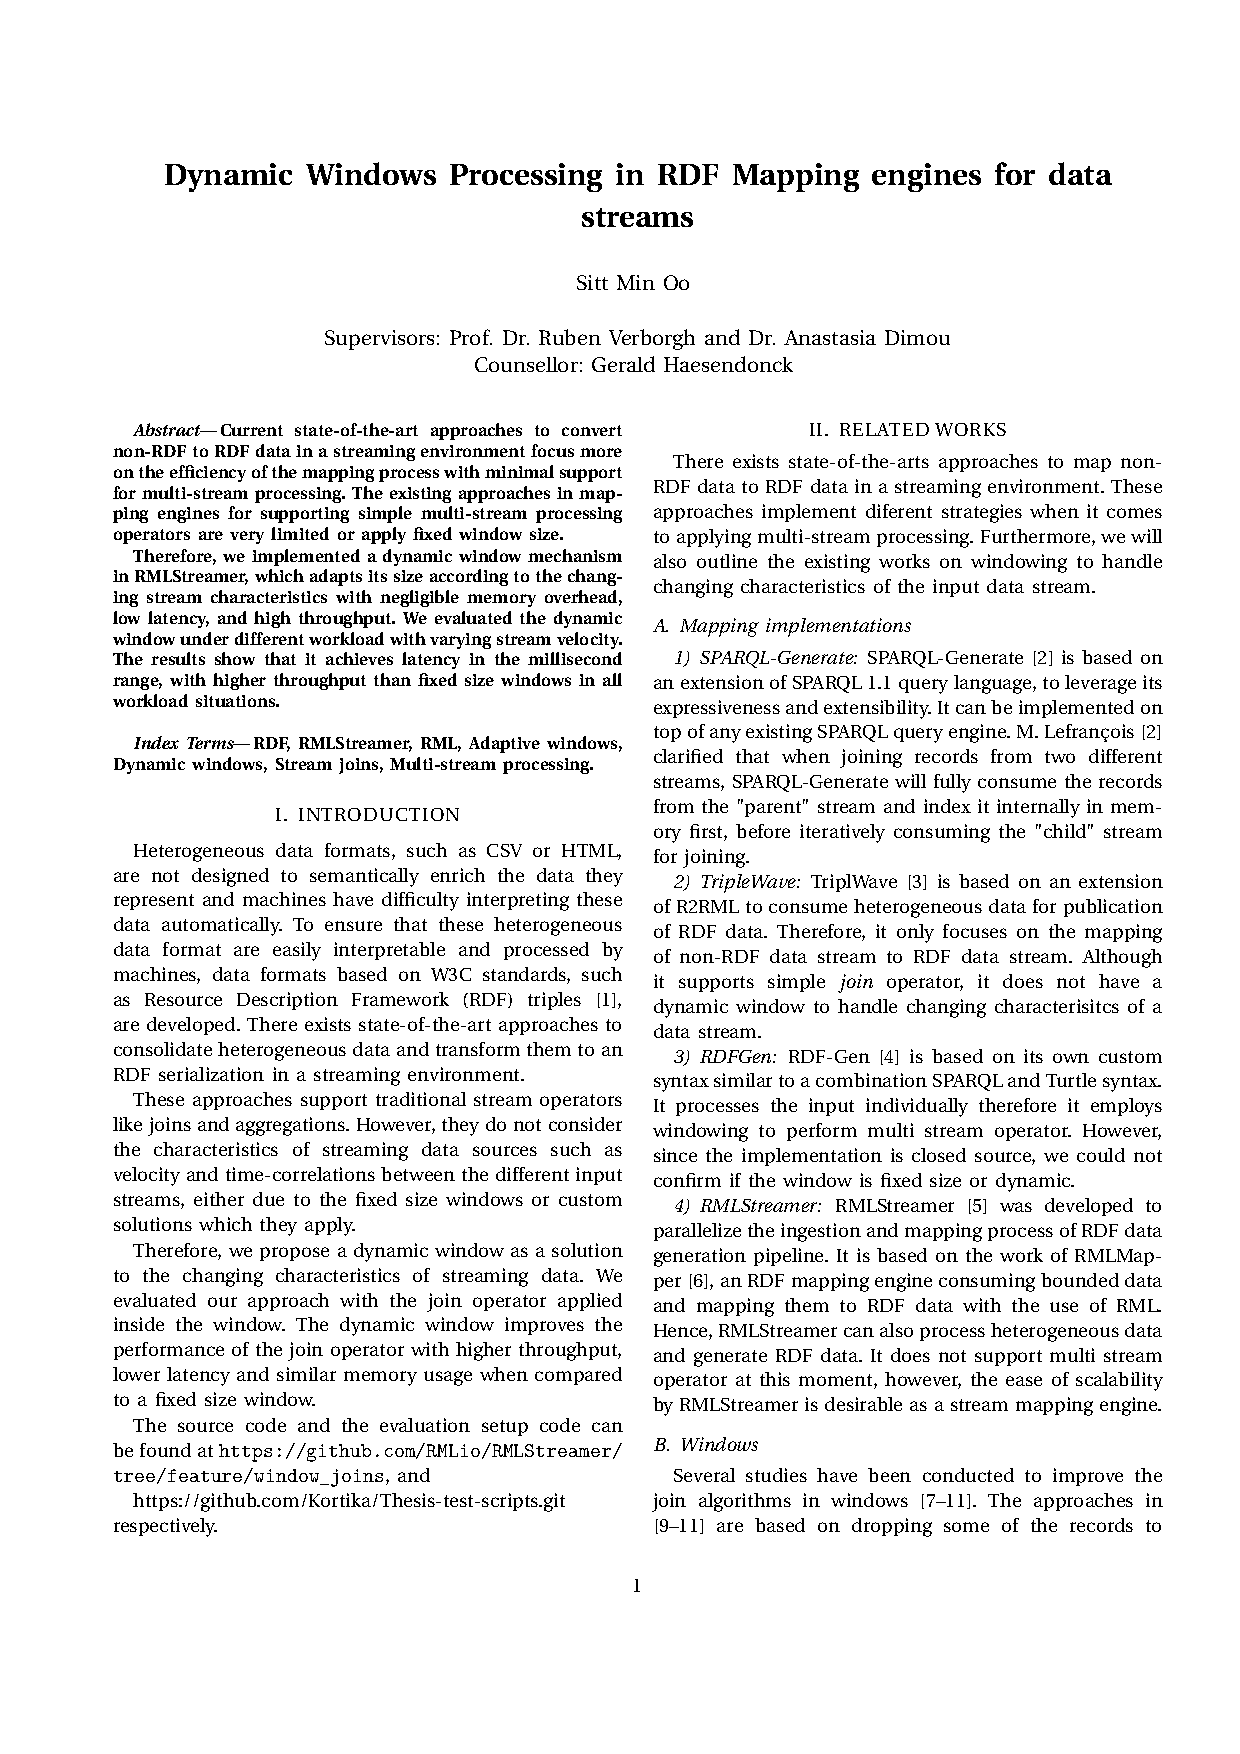
\includepdf[pages=-,offset=75 -75]{abstract.pdf}

\setboolean{@twoside}{true}
\let\cleardoublepage\clearpage

\phantomsection
\addcontentsline{toc}{chapter}{Abstract in Dutch}
\setboolean{@twoside}{false}
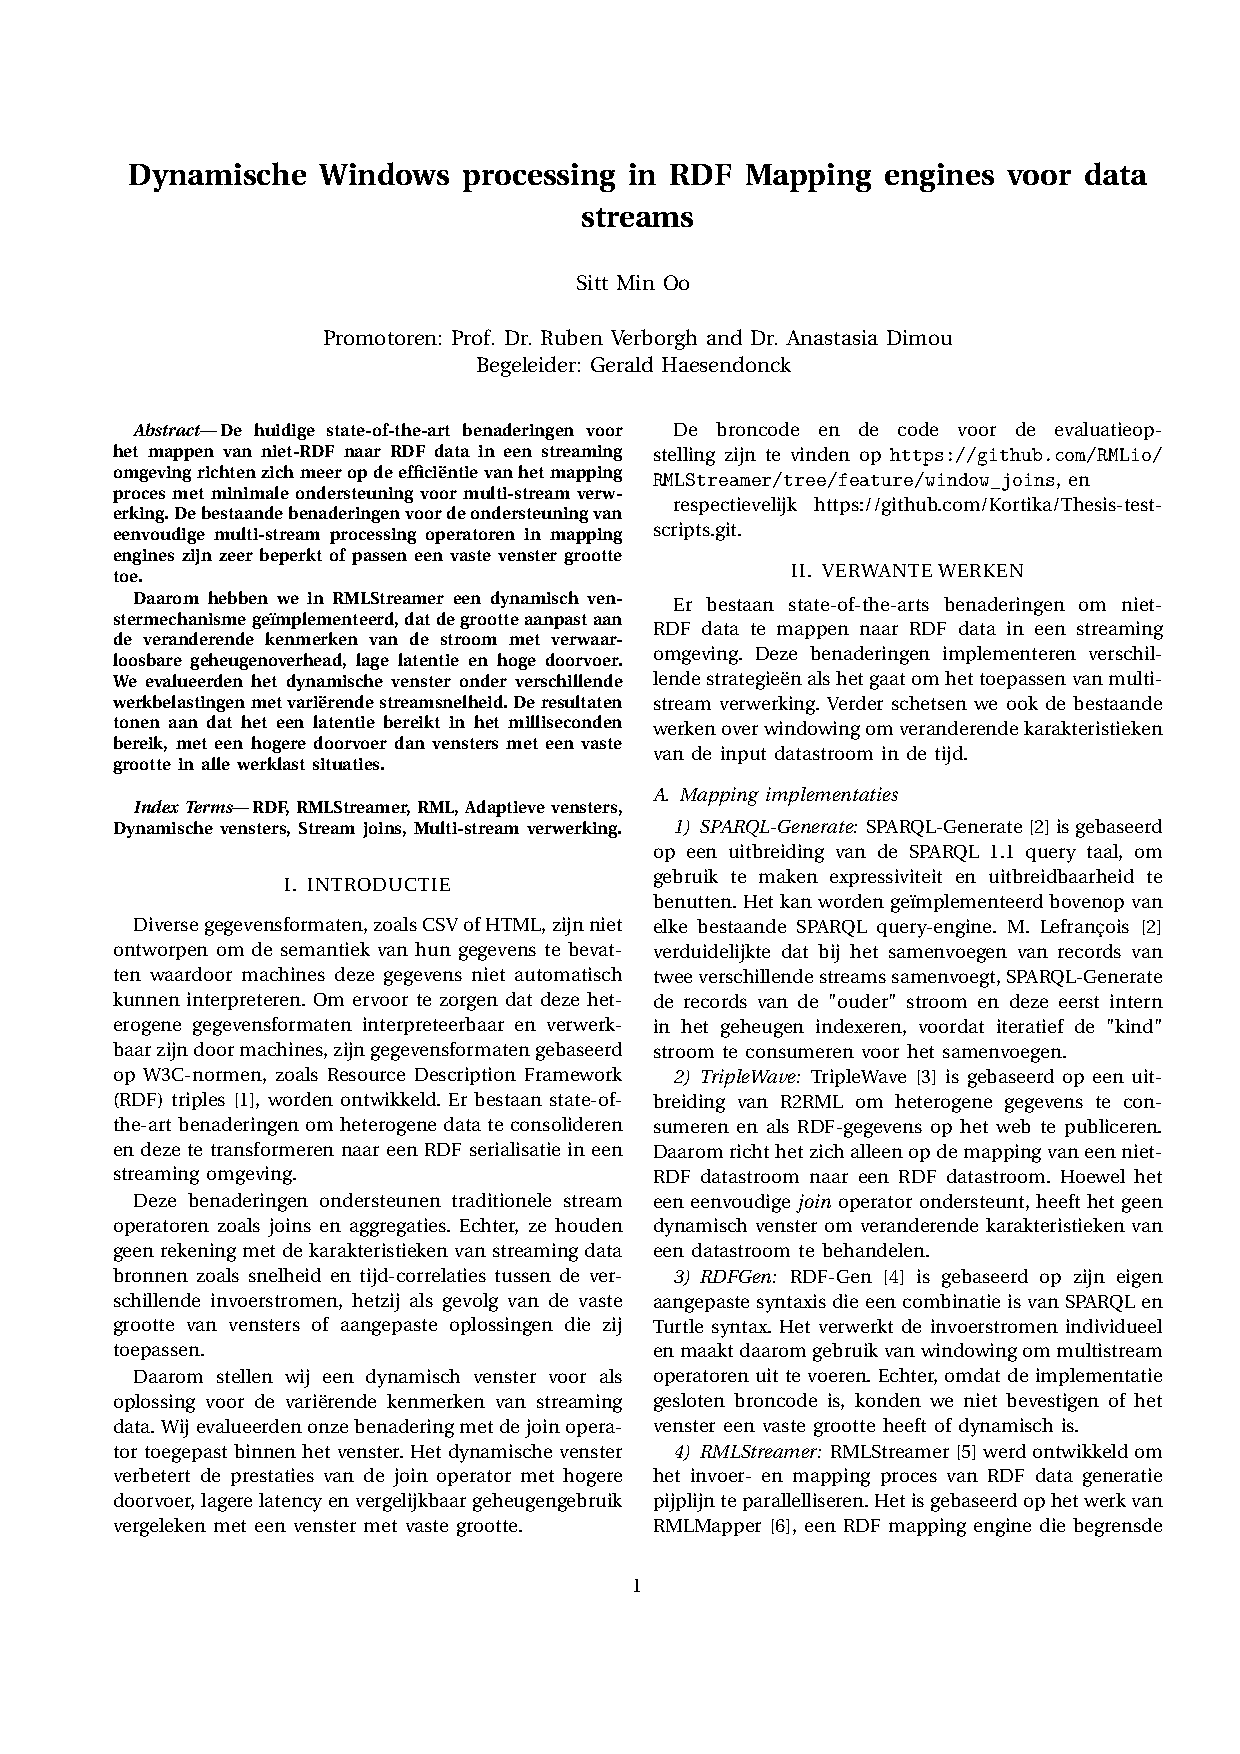
\includepdf[pages=-,offset=75 -75]{abstract_dutch.pdf}

\setboolean{@twoside}{true}
\let\cleardoublepage\clearpage
\pagestyle{fancy}


% toc
\tableofcontents



% optinal makeup
%\setlength{\parindent}{0pt}
%\setlength{\parskip}{0.5\baselineskip plus 0.5ex minus 0.2ex}
%\setlength{\parskip}{1ex plus 0.5ex minus 0.2ex}


\addcontentsline{toc}{chapter}{List of Listings}
\lstlistoflistings
\listoffigures
\listoftables
% chapters
\mainmatter
\setcounter{page}{1}
% add chapters
\chapter{Introduction}
\label{chap:intro}

A large volume of data is generated daily on the Web in a variety of domains. These
data are often structured according to an organization's specific needs or formats: Leading to
a difficulty in integrating the data across the different applications.
These generated data might have to be associated with archival data, also of heterogeneous formats,
to provide a coherent view required by analysis tasks. Heterogeneous Web data formats, such as CSV or HTML, are not explicitly
defined to enable linking entities in one document to other related entities in external documents.

Based on W3C standard, semantic data formats such as RDF triples~\cite{intro_rdf}, are a solution to
this particular problem by enriching the data with knowledge and association across
different domains, through the use of common ontologies. RDF triples also form the basic building blocks of knowledge graphs.
Knowledge graphs are extensively used in social networks like Facebook\cite{facebook_linked_data}, IoT devices\cite{graph_of_things} and especially with Google's search
engine\cite{google_kg}, it enables machines to understand the data and perform complex automated processing
using the knowledge graphs. 

Considering the aforementioned scenarios, there is a need to transform these non-RDF data to RDF compliant formats on the fly while
new data are being generated. Furthermore, we would also like to apply stream operators on the input tuples
before transforming, to enhance the enrichment of the data.

There exists state-of-the-art techniques to solve the task of consolidating heterogeneous data
and transforming them to an RDF compliant format. In this thesis, we will focus on one such format called TURTLE~\cite{turtle_syntax}.
These RDF transformation engines can be categorized into two major categories based on the type of input
which they consume; bounded and unbounded data input. Since we are focussing on the generation of RDF data
in a streaming environment, the class of RDF transformation engines on unbounded data will be of interest to our study.

Some engines support traditional stream operators like joins and aggregations. However, they do not consider
the characteristics of the streaming sources such as velocity and time-correlations between the different
input streams. This leads to a decline in the quality of the generated RDF triples. Moreover,
due to the nature of the infinite, continuous and real-time changing data of the streaming environment,
these operators have to be applied in the context of windows over a subset of the incoming data.
Clearly, with these restrictions and characteristics of the streaming sources, we need an adaptive approach
to applying these operators in windows for the data transformation engines. 

Therefore, we proposed a dynamic approach to windowing for multi stream operators.
The application of these operators in a dynamic window should maintain high memory efficiency and throughput,
even when the velocity of the streaming sources varies greatly over time. 
The dynamic window would make fast and simple statistical calculation to be 
aware of the velocity of the input streams to react and adapt its size accordingly. 
For implementing this dynamic window, we 
\renewcommand{\labelenumi}{(\roman{enumi})}
\begin{enumerate*}
    \item investigate the possible implementation sites which are near the \emph{input}
    or the \emph{output} of the engine, 
    \item provide a reference implementation utilizing the dynamic window, and 
    \item evaluating the implementation against widely used windowing schemes for 
    memory efficiency and throughput. 
\end{enumerate*}


This work aims to improve the performance multi-stream operators, 
by dynamically adapting the window size, according to the dynamic characteristics
of the incoming tuples for the multi-stream operators. Evaluation of 
the implementation is then intended to validate the following hypotheses: 

\begin{hyp}
    Dynamic windows maintain high memory efficiency than 
    fixed size windows even under a dramatic increase or 
    decrease in the velocity of incoming tuples. 
\end{hyp}

\begin{hyp}
    Higher throughput is achieved by multi-stream operators 
    with dynamic windows even with huge delays in the arrival
    rate of tuples between the different streams.
\end{hyp}

Naturally, to further build upon this work, a generic dynamic windowing 
framework could be specified for ease of evaluation and comparison between 
the different dynamic window schemes. Furthermore, we could also define a distributed 
statistical model to build up the characteristics of the streaming sources 
and to automatically apply the appropriate dynamic window. 


The rest of this work will be structured as follows. Chapter~\ref{chap:semantic_web} will 
go over the common terminologies and specifications related to Semantic Web. Readers familiar
with RDF framework and Semantic Web in general, could skip this chapter. 
Chapter~\ref{chap:data_stream_processing} will be about general data stream processing 
and how the state-of-the-art stream processing engines handle multi-stream operators. 
In Chapter~\ref{chap:rdf_data_generation}, current state-of-the-art in 
RDF data generation from non-RDF data sources will be discussed in detail. 
To understand more about windows in stream processing, Chapter~\ref{chap:window_operators}
will go into detail about the current fixed size windows and the other state-of-the-art 
dynamic window operators. 
\chapter{Semantic Web Technologies}


\begin{figure}[htbp]
    \centering
    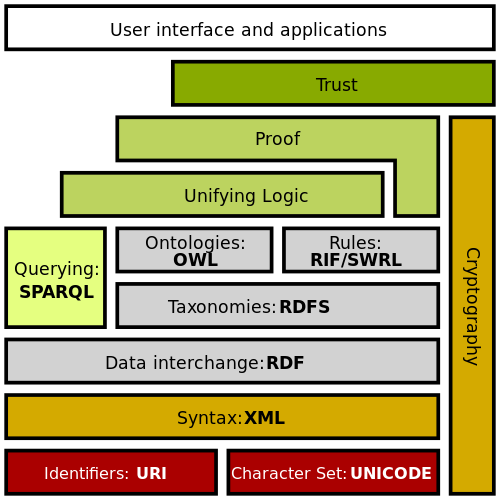
\includegraphics[width=0.5\textwidth]{fig/Semantic_web_stack.svg.png}
    \caption{An overview of semantic web stack with core technologies\cite{sem_web_stack}.}
    \label{fig:sem_web_stack}
\end{figure}

Semantic web extends the existing \emph{web of documents} with the ability 
to \emph{link} different documents and \emph{embed knowledge} in the document
to transform it into a \emph{web of data}. It is perceived by Tim Beners-Lee in 
2001\cite{bernerslee2001semantic} to be integrated into the existing architecture 
of World Wide Web. Embedding \emph{knowledge} into documents enables machines to
interpret the \emph{meaning} of the document and interoperate with each other on 
a more complex level.

Semantic web stack enables one to start building a \emph{web of data} using 
the core technologies shown in Figure~\ref{fig:sem_web_stack}. 
However, this is provided that the data already exists in RDF compliant format.
Existing data on the web in non-RDF format must, therefore, be transformed 
into RDF data enable transition to a \emph{web of data}. This work 
focuses on transforming non-RDF to RDF data, thus the RDF format will be elaborated 
in detail. 



\section{RDF}
Resource Definition Framework \cite{rdf_concepts} is a framework for representing data on the Web.
It portrays the data as a directed graph with the resources as nodes in the graph and the
edges as the relationship between the different resources.
Figure~\ref{fig:rdf_triple_ex} shows an example of an RDF triple statement describing
the information “John has an apple”.
The triple statement consists of the subject \textit{John}, the predicate \textit{has}
and the object \textit{apple}.

\begin{figure}[htbp]
    \centering
    \begin{tikzpicture}[node distance={30mm}, main/.style = {draw, circle}]

        \node[main] (subject) {John};
        \node[main] (object) [right of=subject] {apple};

        \draw[->, thick] (subject) -- node[midway, above, sloped] {has} (object);

    \end{tikzpicture}
    \caption{An RDF triple representing the information “John has an apple”.}

    \label{fig:rdf_triple_ex}
\end{figure}


By composing these simple triple statements into a set of RDF triples, it yields us an RDF graph.
In Figure~\ref{fig:rdf_graph_ex}, 4 triple statements are composed together to form a
simple RDF graph describing \textit{John} and \textit{Mary} having the same \textit{apple}.
\gh{Something is missing from the next sentence:} It might not be evident from the simple figures, about the advantages of
RDF graphs. Data representation in a graph model allows machines to follow the
\textit{links} between the resources, and discover more unknown
data in the linked knowledge graph. \sout{Link following}\gh{Following links} is possible due to the nodes in
the triples being classified as one of the 3 different term types.

\begin{figure}[htbp]
\centering
\begin{tikzpicture}[node distance={45mm}, main/.style = {draw, circle}]

\node[main] (subject) {John};
\node[main] (subject_2) [below of=subject] {Mary};
\node[main] (object) [right of=subject] {apple};
\node[main] (apple_object_colour) [above right of=object] {red};
\node[main] (apple_object_ripe) [below right of=object, text width=15mm] {Malus domestica};
\node [cloud, draw,cloud puffs=10,cloud puff arc=120, aspect=2, inner ysep=1em]
(colour_kg) [below right of=apple_object_colour] {colours KG};

\draw[->, thick] (subject) -- node[midway, above, sloped] {has} (object);
\draw[->, thick] (subject_2) -- node[midway, above, sloped] {has} (object);
\draw[->, thick] (apple_object_colour) -- (colour_kg);
\draw[->, thick] (object) -- node[midway, above, sloped] {has colour} (apple_object_colour);
\draw[->, thick] (object) -- node[midway, above, sloped] {scientific name} (apple_object_ripe);
\end{tikzpicture}
\caption{A simple RDF graph where the same “apple” is shared by both John and Mary.}
\label{fig:rdf_graph_ex}
\end{figure}

\subsection{Term types}
Resources are classified into 3 different term types: IRI (Internationalized Resource Identifier),
literals and blank nodes. \gh{An} \textit{IRI} is a \gh{unique} string identifier \sout{unique} in the global scope to
represent a resource. It is usually in the form of a web address, however, it can
also be in other forms \sout{so}\gh{as} long as it conforms to the syntax defined in
RFC 3987~\footnote{RFC 3987: \url{https://www.ietf.org/rfc/rfc3987.txt}}.
\gh{An} IRI can represent a relationship, a concept or an object. Therefore, it could be
used in the \textit{subject}, the \textit{predicate} and the \textit{object} components of
an RDF triple.

\gh{The} \textit{literal} term type is used to represent a value such as strings, numbers, boolean and dates.
To ensure that the machines know the type of the data being read, we could
explicitly specify the type of the data with a datatype IRI. Moreover, the
language in which the data is written, could also be explicitly stated with
a language tag.

Lastly, we have the term type \textit{blank node}. Blank nodes identify resources
in the local scope (i.e. to a local file or an RDF store). Since it is used to
identify resources in nodes, blank nodes are only applicable as the \textit{subject}
and the \textit{object} components of an RDF triple.


\subsection{Turtle syntax}
\label{sec:turtle_syntax}

\gh{Perhaps briefly explain that there are a number of syntaxes and why you pick Turtle to describe more in detail here}

The aforementioned term types are defined \sout{for}\gh{in the} abstract RDF syntax. For a concrete syntax to write
RDF triples, we would focus on the \sout{TURTLE}\gh{Turtle} (Terse RDF Triple Language)~\cite{turtle_syntax}
syntax in this work. A simple triple statement is a sequence of
\textit{subject, predicate, object} terms, ending in a '.'.
To reduce the repetition of writing the same subject and predicate combination with
different objects, Turtle allows the use of ',' to separate the different objects.
Additionally, one could also use ';' to separate the different predicates and objects sharing the
same subject. 


\begin{lstlisting}[label={lst:same_subject}, 
    caption={Usage of ';' where triples share the same subject.}]
<http://example.org/apple>  <http://example.org/hasColor> "red";
                            <http://example.org/scientificName> "Malus domestica".
\end{lstlisting}

\begin{lstlisting}[label={lst:different_object}, 
    caption={Usage of ',' where triples differs only in the objects.}]
<http://example.org/apple>  <http://example.org/scientificName> "Malus pumila", 
                                                                "Malus domestica".
\end{lstlisting}


IRIs are written between \sout{the} angle brackets like \lstinline{<http://example.org/#John>}.
Since blank nodes are locally scoped version of IRIs, the same syntax to write IRIs is also used.
\sout{TURTLE syntax}\gh{Turtle} allows us to define \textit{prefixes} at the head of the Turtle \sout{file}\gh{document (it can be a file, but also a document on the web for instance)}.
Users could then use prefixes, to write RDF triples in a more compact form. For example,
\lstinline{<http://example.org/#John>} could be shortened to
\lstinline{<#John>} using the relative \textit{@base} path.

\begin{lstlisting}[caption=Prefixes in TURTLE syntax.]
    @base <http://example.org/> . # default base IRI
    @prefix xsd: <http://www.w3.org/2001/XMLSchema#> .
    @prefix rdf: <http://www.w3.org/1999/02/22-rdf-syntax-ns#> .
    @prefix rdfs: <http://www.w3.org/2000/01/rdf-schema#> .
    @prefix foaf: <http://xmlns.com/foaf/0.1/> .
    @prefix rel: <http://www.perceive.net/schemas/relationship/> . 
    ... 
\end{lstlisting}
\gh{I added the xsd prefix to Listing 2.3 because we use it further in the text.}

\sout{Literals are written between the double quote '"'. It has a default datatype of 
a string.}
\gh{A literal is written between double quotes and has by
default the xsd:string datatype} 
One could also \textit{cast} the literal value to a specific datatype 
by appending '\textasciicircum{} \textasciicircum{} $[$IRI of the datatype$]$'. For example, 
"12" is cast to an integer in \lstinline{"12"^^xsd:integer}.
\gh{The} language of the literal value 
can also be specified using \lstinline{@} similarly to datatype casting. 


\chapter{Data Streams} 
\label{chap:data_stream_processing}
With the advent of the \emph{Big Data} era, large amounts of data are being generated 
by companies from their infrastructure; from IoT sensors to events 
generated by customers using online services.
These generated data 
are \emph{unbounded} and infinite, since 
new data are generated continuously. 
For example, the healthcare industry has started to 
adopt the approach of data-driven diagnostics methods~\cite{hospital_diagnosis}. 
This transition is needed to keep up with the increasing amount 
of physiological data generated by the monitoring sensors attached to
patients~\cite{hospital_data_monitoring}. These physiological data are periodically
generated in a continuous streaming manner. 
Consequently, there is a need for 
companies to be able to process these unbounded data streams.

Data Stream Management Systems (DSMS)
are equipped to handle such unbounded data and are adopted 
widely in the industry today in the form of various frameworks such as Apache Flink~\cite{flink} and 
Apache Spark streaming~\cite{spark_streaming}.
The main features of these DSMSs are their ability to 
\renewcommand{\labelenumi}{(\roman{enumi})}
\begin{enumerate*}
    \item scale horizontally, 
    \item process records individually as they arrive, and
    \item process or analyse the data in real time.
\end{enumerate*}

In Chapter~\ref{chap:data_stream_processing}, we will discuss details on  
the characteristics of data streams, how a DSMS typically handles fault tolerance, and
a general strategy to process streaming data. Finally, we will elaborate on
various state-of-the-art frameworks in use by the industry.

\section{Characteristics of Data Streams}
\label{sec:characteristics_data_stream}
What is a data stream? As defined by Golab and Ozsu~\cite{golab_data_stream}:
“A \emph{data stream} is a \emph{real-time}, continuous, ordered (implicitly by arrival time 
or explicitly by timestamp) sequence of items. It is impossible to control the order
in which items arrive, nor is it feasible to \emph{locally store} a stream in its entirety.”

Big Data is usually characterized with the three “V's: \emph{volume}, \emph{velocity} 
and \emph{variety}~\cite{big_data_analytics}.
In the context of data streams processing, it is expected that the data \emph{volume} 
is unbounded since the devices, sensors and applications are constantly 
generating data as long as they are alive. The \emph{variety} aspect of the 
data streams is heterogeneous when different sources 
emit different types of data; structured and unstructured. 
Moreover, \emph{variety} in data can also happen over time; a concept drift where 
the properties of data may change over time unlike Big Data. 


Out of the three aforementioned characteristics, \emph{velocity} is the most important 
factor to consider when it comes to data stream processing. Data in a streaming 
environment are rapidly changing, constantly arriving into the stream processing
pipeline, and need to be processed within a limited time frame.
As a result, only single pass algorithms can
be applied since it is infeasible to have random memory access capability
over the entire stream. Moreover, unlike traditional Big Data processing, 
data stream processing requires \emph{real-time} responses. 
This requirement of low latency processing has the consequence 
that late decisions will result in missing informations. Related to \emph{velocity}, 
the data streams can also have a sudden \emph{'burst'}, a sudden increase in the arrival rate of 
records, which varies over time. 

Monitoring applications of data stream processing are interested in the analysis of 
most recent data. Consequently, the order of the data sequence needs to be considered 
when processing data streams. 
Because data streams are typically transmitted over a 
network, the order of the data cannot be guaranteed. This happens if the network
transmission protocols have no guarantee in the global 
ordering of data or when latency is introduced~\cite{requirements_dsp}. 
In certain applications such as fraud detection in bank transactions and monitoring of 
patient's biometrics, the data streams emitted by the sensors need to be processed in 
real-time. This is because the data streams in such scenarios will rapidly degrade in 
value if they are not handled immediately. Thus, real-time processing of data streams 
is a necessary requirement for data stream processing engines. 

In the context of this work, where we focus on the application of multi-stream operators, 
the \emph{velocity} of a data stream will have a huge impact on the quality and efficiency of 
the generated results. As a consequence of the challenges, as mentioned in 
the example use cases, a Data Stream Management System (DSMS) needs 
to be able to deal with the incoming data appropriately by ensuring that the results are generated 
with low latency, and high throughput without ignoring the timeliness of the data stream.  

\section{Data Stream Management Systems (DSMS)} 
Data Stream Management Systems are designed to overcome the aforementioned challenges 
in data stream processing. Different from the common big data processing, DSMSs should
respond in a limited time frame and process the incoming data with low latency~\cite{data_stream_management}. 
For the former requirement, continuous queries are evaluated repeatedly by the DSMS to react 
to incoming data. The latter can be tackled by reducing the inter-operator communications 
through optimizing operator scheduling and buffers to reduce network traffic~\cite{low_latency_data_stream}. 



\subsection{Fault tolerance}
DSMSs should also scale horizontally 
by distributed stream processing over multiple computing nodes. 
This leads to the requirement that there needs to be some form of coordination and fault tolerance 
for distributed stream processing. The exact details of guaranteeing fault tolerance differs between frameworks, however, there are general strategies to provide some 
form of fault tolerance according to Gradvohl et al~\cite{fault_tolerance_dsms}.
In the context of this thesis, \textbf{fault tolerance} is a crucial requirement when applying
non-trivial operators that are stateful. 
An example of a non-trivial operator would be a recommender algorithm, where 
a user's parameters would need to be kept in the state to update them with each new 
interaction event. This state would then need to be restored in case of failure to 
ensure the proper working of the recommender algorithm.
Another example would be joining streams where a time window is a form of state, 
containing a subset of the data stream. 
The following sections will describe the commonly used strategies to provide fault tolerance 
in DSMS. 

\subsubsection{Replication of components}
Components are operators or computation nodes in the execution pipeline which contains 
some kind of state vulnerable to failure. 
Just as the name suggests, it involves duplicating the components of the stream processing
engine to minimize the error in case of node failures. There are two kinds of replication; 
\emph{active replication} and \emph{passive replication}. In \textbf{active replication,}
duplicated components are executed just like normal components and receive the same incoming data. 
Therefore, there are duplicates in the output --- this allows the engine to check the 
output to identify errors in the normal components. The disadvantage of this method is 
the increase in the cost due to component duplication. 

\textbf{Passive replication} has inactive duplicated components instead. These backup
components are then on standby to replace their counterpart if there is a failure. This 
reduces the performance cost of executing the duplicated components at the same 
time as their counterpart. However, starting the backup component requires the input 
to be resubmitted for it to catch up and return to normal state. This results in a significant 
latency every time there is a failure and not acceptable for the requirement of real-time response. 


\subsubsection{Checkpoint}

Checkpoints represent states the DSMS could be in at a certain point in 
time for each of the input streams, along with the corresponding 
state for each operator. Snapshots of records for each checkpoint are also kept 
by the DSMS to be replayed in case of failure. 
In this fault tolerance strategy, a DSMS is modelled by a sequence of 
checkpoints which are fault free~\cite{fault_tolerance_dsms}. 

In the case of a failure, the operators will be restarted and set back to the state of the 
last successful checkpoint. The records, which were part of the failure, will be replayed
at the input using the snapshot of the state. 

There are two approaches to implement checkpoints at the operator-level; 
\emph{asynchronous} and \emph{synchronous} checkpoints~\cite{fault_tolerance_dsms}.

Uncoordinated checkpoints do not guarantee a global state consistency, since 
each operator performs a checkpoint on their state independently. This results 
in less overhead of saving the state of the whole system with the disadvantage of the higher 
difficulty to revert to a consistent global state.
Figure~\ref{fig:checkpoint_inconsistency}
shows a scenario where uncoordinated checkpoint strategy results in inconsistency of 
global state. In this example, message \emph{m} is not part of the checkpoint of operator 
A even though operator B includes the sending of ~\emph{m} as part of its checkpoint. Therefore, 
rolling back to this checkpoint will result in an inconsistent global state, causing the 
DSMS to roll back to an earlier consistent checkpoint. In the worst case scenario, this could result 
in the DSMS trying to repeatedly roll back until a consistent checkpoint is met, 
resulting in a 'domino effect'.  

On the other hand, in coordinated checkpointing, the operators will take a snapshot 
of their internal state at the same "time" and save them to provide a consistent 
global state, avoiding the 'domino effect' of asynchronous checkpointing. To ensure 
the global consistency, a global synchronization mechanism is required. A simple 
algorithm to achieve this mechanism, is to have a central coordinator to synchronize 
the checkpointing process amongst the different operators. This introduces an overhead 
while coordinating these operators, increasing the latency of the operators whenever a 
checkpoint has to be taken. 


Combined approaches utilizing different operators, such as asynchronous, and non-blocking
operators, exist for checkpointing with the consistency of global states. 
The Chandy-Lamport algorithm~\cite{chandy_lamport} determines the 
global state of a distributed system which could be used to maintain the checkpoints. 

\begin{figure}[!htbp]
    \centering
    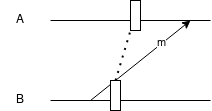
\includegraphics{fig/checkpoint_inconsistency.png}
    \caption{Inconsistent checkpoint scenario where operator A and B have different
    checkpointed states. The rectangle blocks indicate the moment when the operators 
    commit a checkpoint of their internal state. }
    \label{fig:checkpoint_inconsistency}
\end{figure}


\begin{figure}[!htbp]
    \centering
    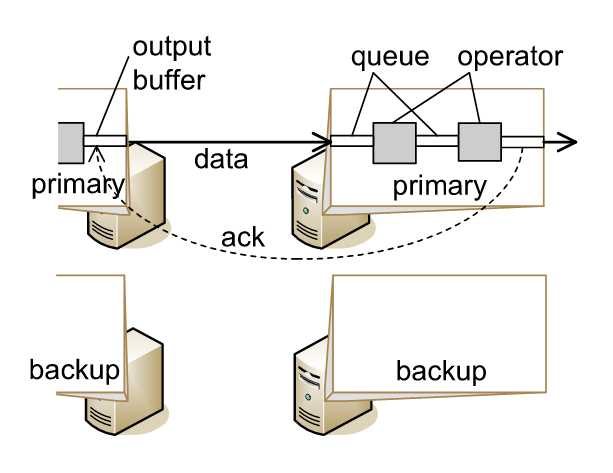
\includegraphics[width=0.5\textwidth]{fig/upstream.png}
    \caption{Upstream backup of the operators for fault tolerance~\cite{upstream_backup}.}
    \label{fig:upstream}
    
\end{figure}

\subsubsection{Upstream backup}

In this approach of fault tolerance, upstream operators 
will temporarily 
keep the records in their output buffer for downstream operators.The records 
stay in the buffer until they are completely processed by the downstream operator. 
The buffer will then be cleared when the upstream operator receives 
an acknowledgement from its direct downstream operators, as illustrated in the Figure~\ref{fig:upstream}. 

The drawback of this approach is that the buffer might not be large enough to 
hold the records stored between the failure and the recovery event. Moreover, 
the whole system needs to be halted until the new operator catches up to 
the state of the failed operator from the replayed records. 

\section{Data Stream processing}

Processing data streams requires a different approach than processing batch data due 
to the characteristics described in Section~\ref{sec:characteristics_data_stream}. 
Batch processing is defined as processing a small subset of the data simultaneously~\cite{batch_processing}. 
Originally, it is meant to tackle a particular characteristic of Big Data; the \textbf{volume}. The job 
could therefore last from several hours to days, depending on the volume of the data and the 
complexity of the operations~\cite{batch_duration}.
Consequently, batch processing engines do not need to take the continuous and 
timely nature of the data into account~\cite{flink}.
On the other hand, stream processing requires the notion of time and continuity of the data 
(Section~\ref{sec:characteristics_data_stream}). This brings several challenges 
that stream processing frameworks need to solve, resulting in a specialised architecture employed by the 
frameworks. In this section, we will summarise the general architecture and strategies to deal with the 
uncertainty of the order of items and the continuously processing of items in data streams. Different 
state-of-the-art frameworks will also be briefly mentioned, to get the reader familiar with the 
frameworks. 

\newpage

\subsection{Lambda architecture}

Batch processing introduces high latency --- if a query 
is executed against a batch processing engine, it can take hours to return the results, which might be 
out of date once they are ready. A combination of the speed of stream processing with the accuracy of batch analysis
allows one to process the unbounded data stream with low latency and maximal accuracy. 

Lambda architecture~\cite{lambda_arch, lambda_arch_book, lambda_arc_bpost} introduced by Nathan Marz, is a 
design pattern to combine the high accuracy of batch analysis and the low latency of 
stream processing engines. It consists of three separate layers; a \textbf{batch} layer, 
a \textbf{speed} layer and a \textbf{serving} layer. 
The three layers serve to enhance the result of the users' queries by taking 
advantage of both the low latency of the \textbf{speed} layer and the accurate analysis of the \textbf{batch}
layer.


To further complement the three layers, 
the data stream is also split into two different paths: 
\begin{itemize}
    \item A \textbf{cold} path --- data flowing in the cold path is not required to fulfil the low
        latency requirement. The \textbf{batch} layer is located along the cold path.   
    \item A \textbf{hot} path --- data along the hot path is constrained by the low latency requirement 
        and needs to be processed at high velocity. Therefore, it flows through the 
        \textbf{speed} layer.  
\end{itemize}

\begin{figure}[!htpb]
    \centering
    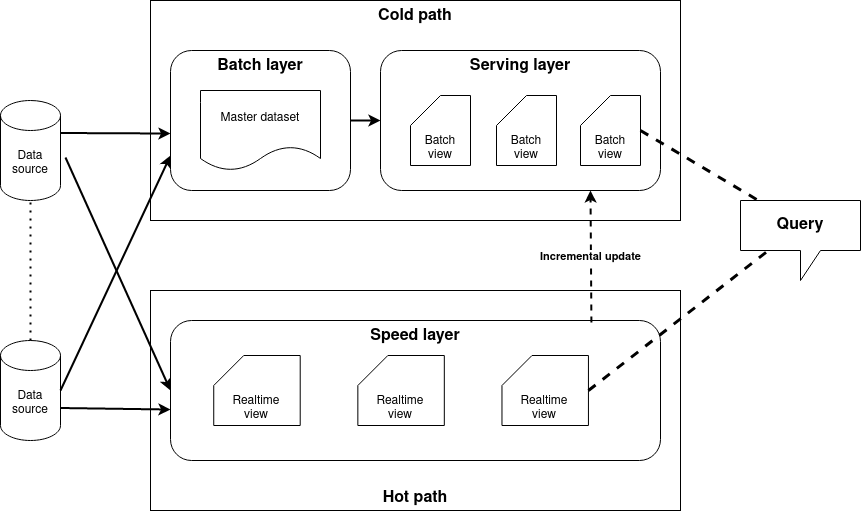
\includegraphics[width=\linewidth]{fig/lambda_arch.png}
    \caption{A general overview of the Lambda architecture. User queries are served from 
    the real-time views until the batch views are ready. Incremental updates could also be applied 
to the batch views in the \textbf{serving} layer by using the results from the \textbf{speed} layer.
~\cite{lambda_arch_book}}%
    \label{fig:lambda_arch}
\end{figure}

\subsubsection{Speed layer}%
\label{sssec:Speed layer}
The speed layer is responsible for processing the incoming data at high velocity and low latency. 
This layer focuses at low latency processing at the cost of a lower accuracy. The generated 
\textbf{real-time views}  could also be used to incrementally update the \textbf{batch views} since they 
are more recent due to low latency processing. Stream processing engines are employed in this 
layer.  \textbf{Windowing operators} are employed 
to restrict the stream processing to the elements contained within the \textbf{window}. 
This ensures that the analysis is done on a subset of the whole streaming data. 
Chapter~\ref{chap:windows} elaborates the different \textbf{windows} that 
are commonly used in stream processing. 

\subsubsection{Batch layer}%
\label{sssec:Batch layer}
The batch layer stores the incoming stream data in a \emph{master dataset}. This \emph{master dataset} is an immutable
and append-only dataset, to ensure that there is some notion of time or history of the data. Changes made to 
the previously stored data are re-appended to the dataset as a record with a new timestamp.  
This enables re-computation of the master dataset resulting in a new batch view as the dataset evolves over time. 
Batch processing engines, such as MapReduce~\cite{mapreduce}-based framework like Apache Hadoop~\cite{hadoop}, 
are commonly deployed the batch layer for batch analysis. 


\subsubsection{Serving layer}%
\label{sssec:Serving layer}

The serving layer receives the batch views from the batch layer and updates them as necessary. When a user 
queries the application, the serving layer will redirect the user to the real-time views if the 
requested data needs to be timely. Otherwise, the batch views will be returned to the user which are 
more accurate but less timely.  


\subsubsection{Summary}%
\label{ssub:Summary}

Separating the whole processing system into two separate components along 
the two different data paths, the \textbf{batch} layer on the \textbf{cold} path, and 
the \textbf{speed} layer on the \textbf{hot} path, introduces complexity in maintaining the business logic of the system.
If 
there is any change in the type of analysis done in one layer, the other layer needs to be updated 
with the corresponding batch analysis task. Therefore, there is unnecessary complexity in managing 
the system along the two dataflow paths. 
    

\subsection{Kappa architecture}%
\label{sub:Kappa architecture}
Kappa architecture~\cite{kappa_architecture}, as proposed by Jay Kreps, 
combines batch and stream processing into one layer, to replace the 
two processing systems layout of the Lambda architecture. Intuitively, stream processing is 
only meant to handle a very small subset of the whole data. However,
one could increase the parallelism of the streaming 
job and reprocess the whole historical data as a \emph{subset}, by replaying 
the historical data at high velocity. This results in an output accuracy as 
batch analysis. The Kappa architecture is based on this intuition.   
Instead of consuming the streaming data sources directly with the stream processing engine, 
the input data is first stored in a distributed data log system like Apache Kafka~\cite{kafka}. The data 
logs can be stored indefinitely or temporarily depending on the use case.
The stream processing layer has access to the data in two forms; 
a stream of events in real-time, or as a replay of historical data for batch analysis. 

\begin{figure}[!htbp]
    \centering
    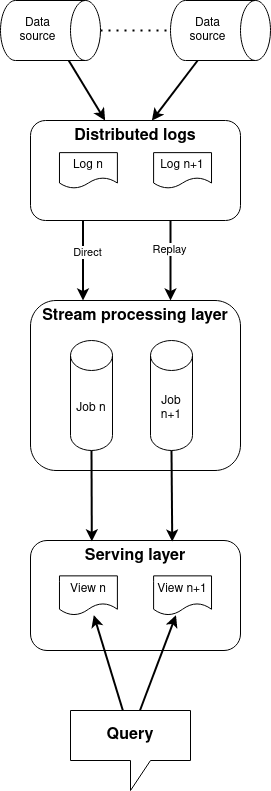
\includegraphics[width=0.4\linewidth]{fig/kappa_arch.png}
    \caption{An overview of the Kappa architecture. Here, job \emph{n+1} is re-processing using the replay 
    data from the unified data logs in parallel. Once it has caught up to the output of job \emph{n}, 
    job \emph{n} can be phased out and allow the latest job \emph{n+1} to take over.}
    \label{fig:kappa_arch}
\end{figure}


\subsubsection{Summary}%
Even though the Kappa architecture solves the problem of code redundancy and complexity of 
system management introduced in the 
Lambda architecture, it is not meant as a full replacement for the Lambda architecture. 
The Lambda architecture is useful in cases where two different algorithms for 
batch analysis and stream processing are needed. For example, the batch layer could be responsible for training 
a machine learning model on the bounded dataset batches and improving the 
predictions, while the speed layer could deploy these models to provide real-time predictions. 


In this thesis, we investigate the usage of dynamic windows in the context of stream processing 
heterogeneous data to RDF data. 
Therefore, the Kappa architecture is the best candidate to deploy and test our 
hypotheses since we have no need for batch analysis in this thesis.  

\subsection{Out-of-order processing}%
\label{sub:Out of order processing}
Stream events can arrive out-of-order due to a myriad of reasons; network latencies, 
bad connections or a delay at one of the multiple sensors generating the events for 
the stream processing engine. Stream 
processing engines should be aware of the \emph{timeliness} of the data stream --- it needs 
to be able to deal with out-of-order events. 

To understand the strategy involved in the handling out of order events, 
two notions of \emph{time}~ need to be introduced~\cite{watermark_flink}:  

\begin{defn}[Processing time]
    Processing time refers to the time of the system on which the stream processing 
    engine is being executed. The system clock of the machine is therefore used 
    to mark the \emph{processing time}. 
\end{defn}
Marking events with processing time makes them 
susceptible to the speed and the order in which they arrive in the system. 
In a distributed environment, on which stream processing engines are often 
executed, processing time does not provide determinism. This is because 
reprocessing the same set of data stream will not lead to the same output, if 
the two execution are executed in sequence, since the processing time will be 
different, resulting in different watermarks. 


\begin{defn}[Event time]
    Event time is the time at which the events are generated at the source.
\end{defn}
For example, the \emph{event time} of a user's click events,
will be the exact time the user \textbf{clicks} on an object of 
interest. This timestamp is usually included in the record as they arrive 
in the stream processing engine. The engine could then extract these 
timestamp to use as \emph{event time}. 


\subsubsection{Watermarking}%
\label{ssub:Watermarking}

The two notions of \emph{time} are used in a strategy called \textbf{watermarking}~\cite{watermark_millwheel}. 
Watermarks are timestamp thresholds used to deal with \emph{very late} events 
in the data stream. It specifies how long the stream processing engine 
waits for \emph{late events}. For example, if a watermark with timestamp 
20 arrives in the dataflow, the system could assume that all events 
with timestamp earlier than 20 already have arrived in the system. 

Notions of time and watermarks are insufficient to handle out-of-order 
events. The stream processing engine needs to be able to compare them to a subset of the 
incoming data. Windowing provides a grouped view of the infinite unbounded stream, 
enabling the engine to compare the subset of records for \emph{timeliness} and out-of-order 
processing. A window can be \emph{time driven}, every $N$ seconds, or \emph{data driven}, 
every $N$ records. 
In Figure~\ref{fig:watermark}, a time window is applied on the stream that
stretches from watermark \emph{W(17)} until \emph{W(11)}. 
Once \emph{W(17)} arrives in the window, it knows that it contains or has 
processed all events earlier than timestamp 17 and later than timestamp of 11.  

However, future events may arrive in the window 
with a timestamp earlier than 17. That event can be considered \emph{late} as an outlier and 
be dealt with appropriately as defined by the developer. Different windows 
behave differently with the watermarking strategy. Chapter~\ref{chap:windows}
will elaborate the workings of different windows and how windowing works in 
general. 


\begin{figure}[htpb]
    \centering
    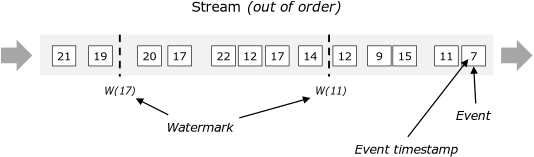
\includegraphics[width=0.8\linewidth]{fig/stream_watermark_out_of_order.png}
    \caption{Out of order events in a stream with watermarks~\cite{watermark_flink}. In this figure, 
    all events on the right side of W(11) have a timestamp $\le 11$. If an event with 
    a timestamp $> 11$ arrives in the future, it is considered \emph{late}.}
    \label{fig:watermark}
\end{figure}


\section{Frameworks}
\label{sec:frameworks}
There are various state-of-the-art stream processing frameworks widely employed
in the industry. These frameworks address the main challenges of 
Big Data stream processing, the three V's (Section ~\ref{sec:characteristics_data_stream}),
differently with their own advantages and disadvantages.

In this section, we elaborate 
on a few of these stream processing frameworks to identify the best characteristics of a 
stream processing engine and the different implementations to tackle the challenges by these 
frameworks.



\subsection{Apache Spark Streaming}%
\label{sub:Apache Spark}
Apache Spark~\footnote{Apache Spark: \url{https://spark.apache.org/}} is a batch 
processing framework developed to improve upon the existing implementations of the 
MapReduce paradigm. Spark processes data in RAM with a read-only data structure called 
\emph{Resilient Distributed Dataset} (RDD) instead of working purely with a distributed file based system like 
Hadoop. RDD is distributed over 
different machines in the cluster allowing parallel operations. Fault tolerance 
is also enabled through incremental bookkeeping of how RDD is built over time, allowing 
it to be rebuilt in case of failure.

These RDDs are the crucial building block to implement the stream processing engine 
based on Spark; Apache Spark Streaming~\cite{spark_streaming}. Spark Streaming structures
stream processing as a series of \emph{stateless, deterministic micro batch
computations} on small interval times~\cite{spark_streaming}. Discretizing the stream 
into micro batches frees up the stream processing engine from synchronization protocols 
and dependency of the data across time. Since the stream is modelled as \emph{micro} 
batches, the powerful recovery mechanisms and exactly-once delivery semantics of the traditional batch processing engines could
be applied. 
Furthermore, transparent integration of RDDs for both batch and stream processing in Spark,  
means that Spark Streaming utilizes the Kappa architecture to maintain low latency stream processing. 

However, Apache Spark Streaming still has a 
higher latency compared to systems processing individual records in the stream, 
such as Apache Flink and Apache Storm, due to the discretization of 
data stream in \emph{micro} batches. 


\subsection{Apache Storm}%
\label{sub:Apache Storm}

Apache Storm~\footnote{Apache Storm: \url{https://storm.apache.org/}} is 
created by Nathan Marz.
Storm's architecture 
consists of \emph{streams of records} flowing through
\emph{topologies}~\cite{storm_twitter}, in comparison to 
the micro batches structure of the stream in Spark Streaming. 
This is a structure where operators are 
represented as \emph{nodes} and the data flow between these operators as \emph{edges} of 
a directed acyclic graph (DAG) as shown in Figure~\ref{fig:dag_topology}. 
The \emph{nodes} are further distinguished between 
two main functions; \emph{spouts} (data sources) and \emph{bolts} (computations).  
By processing the stream events as individual records, the latency is kept 
to a minimum in the \emph{bolts}. 

Storm provides at-least-once 
delivery semantics through the use of record-level acknowledgements. A randomly 
generated "id" is attached to each new record and an extra \emph{acker node} is attached 
to the execution graph. This \emph{acker node} is responsible for tracking the records, 
enabling at-least once delivery semantics. Storm could be upgraded to enable 
exactly-once semantics with the utilization of an API called
Trident~\footnote{Trident API: \url{https://storm.apache.org/releases/2.1.0/Trident-API-Overview.html}}. 
However, Storm would then structure the stream events as mini batches just like 
Spark Streaming, forfeiting the low latency processing. 

Implementing computation tasks 
in Storm is non-trivial, due to its low-level definition of the \emph{bolts}, 
and requires the implementation of one or more readers and 
collectors. This results in non-intuitive composition of the execution topology. 
Furthermore, Storm does not support 
batch processing, offering no options to extend the functionality of the stream 
processing application if batch processing support is required in the future. 


\begin{figure}[!htpb]
    \centering
    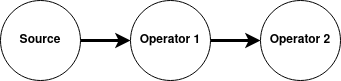
\includegraphics[width=0.5\linewidth]{fig/dag.png}
    \caption{A common stream processing topology representation as a DAG where the 
    dataflow is represented as the directional edges between de operators.} 
    \label{fig:dag_topology}
\end{figure}

\subsection{Apache Flink}%
\label{sub:Apache Flink}

Apache Flink~\cite{flink} aims to bridge the gap between batch and stream processing aspects of 
Big Data and combine them into one unified framework. Similar to Storm, 
Flink's execution topology is also internally represented as a DAG (Figure~\ref{fig:dag_topology}).
It also processes the incoming records as 
individual events to maintain low latency processing. Flink recognizes that
dedicated batch processing is still needed for applications where no efficient algorithms 
exist for performing the same analysis on streaming data. Therefore, Flink implements a 
specialized API for batch processing on top of its streaming processing engine.

Due to the focus on both batch and stream processing, Flink fulfils the use cases for which 
Spark and Storm specializes in; batch processing and stream processing respectively. Furthermore, 
Flink provides exactly-once delivery semantics, overcoming the need to filter out duplicate 
results and calculation. This is achieved by implementing a variation of the \emph{Chandy-Lamport} algorithm
called \emph{Asynchronous Barrier Snapshotting} (ABS)~\cite{asynchronous_barrier}.
It is much more lightweight than Storm's record-level 
acknowledgements for both fault tolerance and exactly-once delivery semantics
due to the usage of in-stream barriers.  

Finally, Flink provides high-level APIs that make development easier for developers in 
the style of functional programming; an intuitive style for the use cases in the data analysis community. 
Windows are supported in Flink as an integral part of the engine with easy to use high-level APIs for 
commonly used windows (elaborated more on in Chapter~\ref{chap:windows}).  
It also provides access to low-level APIs to implement highly customised windowing logic, without burdening 
the developers with the complexity of the internals of Flink. 
With the ease of development, the aforementioned low latency, and exactly-once delivery semantics, 
Flink is the best candidate to move forward with the implementation of dynamic windows for this thesis. 

\chapter{RDF data generation from non-RDF data}
\label{chap:rdf_data_generation}

How do we generate RDF data from non-RDF data? A variety of specifications and languages exists
which define the generation of RDF data from non-RDF data. These specifications and languages can be grouped 
into two major groups; query languages and mapping languages. Several state-of-the art implementations, 
utilizing these two groups of languages, exist to generate RDF data from non-RDF data.

The implementations could be categorized into two groups; \emph{query-based} and 
\emph{rule-based} implementations. These can be further categorized into two more subgroups 
based on the data that they consume; \emph{bounded} and \emph{unbounded} data. As mentioned in Chapter~\ref{chap:intro}, this work will focus on 
implementations working with unbounded data in a streaming environment, thus implementations 
consuming bounded data will not be elaborated. Before we dive into 
the details of the implementations, we need to elaborate more on the \emph{languages} these implementations 
employ to transform non-RDF to RDF data. 


\section{SPARQL Query Language}
Query languages such as SQL~\cite{sql} already exist in established relational database systems such as 
MySQL or PostgreSQL. It allows users to manipulate and retrieve data 
from relational databases using concise statements. Due to its widespread 
use in the industry for querying databases, it is important that a similar 
query language is used for RDF datasets to ease the transition for the users. 

SPARQL~\cite{sparql} achieves this goal by emulating  SQL to allow 
a seamless transition to RDF by existing data engineers. 
Similar to relational databases, RDF 
datasets can be considered as a table consisting of three columns --- the \textit{subject} column, 
the \textit{predicate} column, and the \textit{object} column. Unlike relational databases, 
RDF datasets, in a table representation, allow the object column to be of heterogeneous datatype. 
Recall from Section~\ref{sec:turtle_syntax}, one could explicitly specify the 
datatype of the object term which allows the heterogeneity in the object column.


Also, different from SQL, SPARQL allows matching based on \emph{basic graph patterns} composed 
of a set of \emph{triple patterns}. Triple patterns are similar to the triple statements 
as clarified in Section~\ref{sec:turtle_syntax} but extended with declared variables (i.e. \emph{?variable\_name}). 
The declared variables are then bound to the concrete value in the corresponding \emph{triple statements},
matching the given \emph{triple pattern}, from the RDF dataset. 
The result of a SPARQL query is returned as an RDF sub-graph of the queried RDF dataset. 

Now a question definitely gets raised in our mind, how does this relate to transforming an 
unbounded dataset to RDF format in a streaming environment? There exists state-of-the-art 
engines for generating RDF data from heterogeneous streaming data sources, which will be 
elaborated in Section~\ref{sec:query_based_implementations}. 

\begin{lstlisting}[language=SPARQL,
    caption={Example of a SPARQL query of a medication.}, 
    label={lst:sparql_example}]
    SELECT ?medication
    WHERE {
      #Basic graph pattern consisting of 2 triple patterns. 
        ?diagnosis example:name "Cancer" .
        ?medication example:canTreat ?diagnosis .
    }
\end{lstlisting}


\begin{table}[htbp]
    \centering
    \begin{tabular}{|c|}
    \hline
    \textbf{medication}        \\ \hline
    Radiation therapy \\ \hline
    \end{tabular}
    \caption{Result of executing the SPARQL query in Listing~\ref{lst:sparql_example}}
    \label{tab:sparql_result}
\end{table}


\section{RDF Mapping Language}
RDF Mapping Language~\cite{rml} is a superset of the W3C's R2RML~\cite{r2rml} which maps relational databases to
RDF datasets. RML improves upon R2RML by expressing mapping rules from heterogeneous
data sources and transforming them to RDF datasets whereas R2RML could only consume
data from relational databases. An RML mapping document is composed of one or more \emph{triples maps}, 
which in turn consist of \emph{subject, predicate} and \emph{object} term maps. As the names imply, 
the term maps are used to map elements of the data sources to their respective terms 
in an RDF triple. The definitions of these maps are similar to the 
specifications in R2RML~\cite{rml_tech}. 

Logical sources could be defined by specifying the \emph{source, logical iterator} 
and zero or one \emph{reference formulation} property.
Although the reference implementation RMLMapper could only process logical sources 
consisting of bounded data, the expressiveness and the flexibility of RML allows one 
to extend it to support unbounded data sources. For example, RMLStreamer~\cite{rml_streamer} implementation in 
Section~\ref{sec:rml_streamer} extended the base RML vocabulary to support logical sources with unbounded data. 

RML also supports defining relationships amongst the different 
triples maps through the use of \textit{rr:parentTriplesMap, rr:joinCondition, rr:child and rr:parent}
properties. Different triples maps might come from separate logical sources, therefore, 
referencing across triples maps might require applying the join operator across multiple 
logical sources. 

Moreover, an ontology to semantically define functions, FnO~\cite{fno_ben}, has been supported 
in RML, allowing users to apply user defined functions during the mapping process. This 
extension provides RML implementations with the capabilities to transform the input data with 
lightweight computations before mapping them into RDF triples; providing some form of 
data processing. 

\begin{lstlisting}[caption={An example of an RML mapping document~\cite{rml_tech}}.]
@prefix rr: <http://www.w3.org/ns/r2rml#>.
@prefix rml: <http://semweb.mmlab.be/ns/rml#>.
@prefix ex: <http://example.com/ns#>.
@prefix ql: <http://semweb.mmlab.be/ns/ql#>.
@prefix xsd: <http://www.w3.org/2001/XMLSchema#>.
@prefix rdfs: <http://www.w3.org/2000/01/rdf-schema#>.
@base <http://example.com/ns#>.

<#TransportMapping>
  rml:logicalSource [
    rml:source "Transport.xml" ;
    rml:iterator "/transport/bus/route/stop";
    rml:referenceFormulation ql:XPath;
  ];

  rr:subjectMap [
    rr:template
      "http://trans.example.com/stop/{@id}";
    rr:class ex:Stop
  ];

  rr:predicateObjectMap [
    rr:predicate rdfs:label;
    rr:objectMap [
      rml:reference "."
    ]
  ].
    
\end{lstlisting}

\section{Query based implementations}
\label{sec:query_based_implementations}

When we think of interacting with a data source, querying the data source with a 
query language seems natural since that is the common method to interact 
with a database. Allowing users to query the sources without explicitly 
defining the mapping semantics hides the mapping or data transformation details from the user. 
Moreover, it eases the transition to developing applications using RDF data since the syntaxes are 
similar to the existing query languages leading to lower learning curve for the developers.
To the best of our knowledge, there exist two state-of-the-art 
template based implementations, using SPARQL query-like languages, for transforming 
unbounded non-RDF data to RDF data: SPARQL-Generate and RDF-Gen.
These engines will be elaborated more in the following sections.


\subsection{SPARQL-Generate}
SPARQL-Generate~\cite{sparql_generate} was proposed as an alternative to then existing methods of 
transforming non-RDF data. The language is based on an extension of SPARQL 1.1 query language, to leverage 
its expressiveness and extensibility. Furthermore, this allows SPARQL-Generate to be implemented on top 
of any existing SPARQL query engine. The reference implementation in the paper was based on Apache Jena's 
SPARQL 1.1 engine. Due to the use of the existing SPARQL 1.1 query language, experienced knowledge engineers could use 
SPARQL-Generate to improve the generation of RDF data in their existing workflow. 

SPARQL-Generate supports the consumption of heterogeneous data sources by exposing the 
\emph{binding} and \emph{iterator functions API}. Therefore, covering a new data format or data source could be accomplished 
by implementing the corresponding \emph{binding} and \emph{iterator functions}. Currently, as of writing this paper, 
the reference implementation supports the consumption of data sources which are unbounded and in a streaming environment. 
For example, WebSocket and MQQT are currently supported in the latest version of SPARQL-Generate. 

Although there is a support for data stream processing, the paper did not go into details 
about the application of multi-stream operators like joins when involving multiple streaming 
data sources. The author, M. Lefran\c{c}ois, clarified that when joining
records from two different streams, SPARQL-Generate will fully consume the records 
from the "parent" stream and index it internally. The "child" stream will then be iteratively consumed and 
joined with the records from the internal index. Hence, we could assume that SPARQL-Generate processes the "parent" 
stream in memory when there is a multi-stream operator.
Furthermore, the 
authors mentioned that SPARQL-Generate could use the SPARQL 1.1 operators such as \emph{join operators}. 
From this, we could derive that SPARQL-Generate will apply \emph{join} on the 
records by delegating it to the underlying SPARQL engine.
Therefore, there is a lack of  
dynamic windowing schemes to efficiently exploit the characteristics of the streaming data sources.  

\subsection{RDF-Gen}
RDF-Gen~\cite{rdf_gen} is also based on SPARQL-like syntaxes. However, instead of extending SPARQL engines, 
it provides its own architecture as laid out in Figure~\ref{fig:rdf-gen-arch} to meet the demands
of real-time processing. Instead of adopting most of the syntax from SPARQL, RDF-Gen only 
keeps the basic graph pattern section of SPARQL query to reduce the size of the transformation specification. 
Thus, it has the most compact mapping template compared to the other methods mentioned in this paper. 

RDF-Gen consists of three main components: 
\begin{enumerate*}[label=(\alph*)]
  \item Data Connector,
  \item Triple Generator, and
  \item Link Discovery.
\end{enumerate*}

Data Connectors allows close-to-source processing, 
which is not the case for SPARQL-Generate. This is due to the data consumption 
module being tightly coupled with the mapping process for SPARQL-Generate, unlike 
RDF-Gen as shown in Figure ~\ref{fig:rdf-gen-arch}. 
Triple Generator handles the rapid generation of RDF triples by making use of 
template graphs and variable vectors. The Link Discovery component solves the 
problem of link discovery problem which is defined as follows:
Given two data sources $S$ and $T$, the problem is to find the pairs of elements in 
$S \times T$ that are related to each other (e.g. following the predicate of 
\emph{owl:sameAs} property). Since we are concerned with 
multi-stream operators during RDF generation in this paper, link discovery component could be ignored. 


\begin{figure}[!htbp]
  \centering
  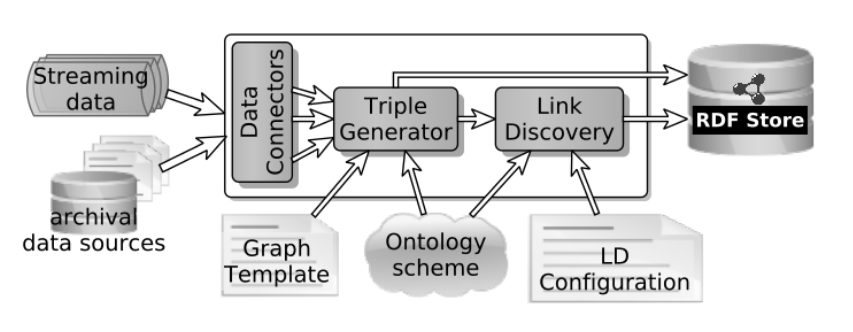
\includegraphics[width=0.8\textwidth]{fig/rdf-gen-arch.png}
  \caption{Architecture of RDF-Gen~\cite{rdf_gen}}
  \label{fig:rdf-gen-arch}
\end{figure}

\subsubsection{Data Connector}
Data Connector has a similar functionality as the \emph{iterator functions} from SPARQL-Generate.
It consumes the data sources given a configuration setting. The configuration setting is used to specify 
the type of data sources, the \emph{window} for processing the incoming data records and 
also apply functions on the incoming data elements. Data Connector can thus be defined as a 
mapping function as in Definition~\ref{defn:data_connector}. 


\begin{defn}[Data Connector record~\cite{rdf_gen}]
  \label{defn:data_connector}
  Given a set of data sources $D = \{d_1, d_2, \dots, d_n\}$ and  a 
  mapping function $F = \mu_{f}(d_i, e)\; |\; \forall d_i \in D$ with $e$, a data element 
  of a data source $d_i$, and $f$, a filter function. Data Connector 
  generates a record $R = \mu_{f}(d_i, e)$ $\iff$ all the attributes of 
  $e$ satisfy the filter function $f$. By default, the filter function $f$ just returns true. 
\end{defn}

Using the Definition~\ref{defn:data_connector}, we could now also apply an equi-join operator 
on the data sources. Formally, we could generate a new triple 
$R =  \mu_{f_i}(d_i, e_i) \bowtie  \mu_{f_j}(d_j, e_j) $ where $e_i$ and $e_j$ have 
common attributes under the filter functions $f_i$ and $f_j$. 

The processing is done on individual records, leading to 
RDF-Gen treating streaming and archival data sources the same way --- as “streams” 
of records. Due to the record-by-record processing, the framework also has a very low 
memory usage. 

\subsubsection{Triple Generator}
As indicated in Figure~\ref{fig:rdf-gen-arch}, Triple Generator consumes the output records 
of the Data Connectors to convert them into RDF triples. A vector of variables $V$, an RDF 
graph template $G$, akin to the basic graph pattern from SPARQL 1.1, and a 
set of \emph{functions} $F$ can be used to configure the Triple Generators. 

$V$ consists of variables which corresponds to the attributes of the
generated records from the Data Connector. These variables are referenced 
in the graph template $G$, and then used to 
bind to the attribute value of the record provided by the Data Connector. 
In case these variables are the arguments of a function $f \in F$, the function will 
be evaluated and the result appended to the output. Therefore, 
this simple binding of values in a template graph enables Triple Generator to 
generate RDF triples efficiently and have a high scalability. Generally, to 
keep the computational time low, the functions will have to be simple in complexity. 


Next, we shall work on a small example to understand how Triple Generator works. 
Listing~\ref{lst:rdf_gen_example} shows an example of a graph template $G$ provided to 
the Triple Generator to generate RDF triples. In this example, the provided vector 
of variables is $V = [\textrm{?diagnosis\_id}, \textrm{?name} ]$. If the incoming record 
is as shown in Table~\ref{tab:rdf_gen_sample_record}, the specified variables,
\emph{diagnosis\_id} and \emph{name}, will be bound to the values \emph{100} and 
\emph{Cancer} respectively. Afterwards, the functions \emph{makeUri} and \emph{asString} will 
be called with the bounded values as arguments and the generated 
output will be used to generate the RDF triples specified by 
the graph template. 
The final generated set of RDF triples is (e.g. in turtle syntax): 

\begin{lstlisting}
  ... 
  <http://example.com/100>  a example; 
                            example:name  "Cancer". 
  ...
\end{lstlisting}


\begin{table}[!htbp]
  \centering
  \begin{tabular}{l|l}
  \multicolumn{1}{c|}{\textbf{diagnosis\_id}} & \multicolumn{1}{c}{\textbf{name}} \\ \hline
  100                                 & Cancer                    
  \end{tabular}
  \caption{A sample record generated by the Data Connector.}
  \label{tab:rdf_gen_sample_record}
  \end{table}

\begin{lstlisting}[language={SPARQL},
   caption={A simple graph template $G$ with the functions \emph{asString} and \emph{makeUri}.}, 
   label={lst:rdf_gen_example}
  ]
  #BGP for the diagnosis data source
  makeUri(?diagnosis_id)  a example:Diagnosis;
                          example:name asString(?name).
\end{lstlisting}

Consumption of input on a record-by-record basis results in RDF-Gen having to 
handle multi-stream operators with the use of windows. However, the paper did not 
mention in detail about its implementation of windows to handle 
multi-stream operators since it was out of scope. Therefore, we still have no 
notion of how to handle data streams with dynamic characteristics where fixed windows 
size have negative consequences on the quality of the generated RDF data. 


\section{Mapping based implementations}
\label{sec:mapping_based_implementation}
Other than approaching the transformation of non-RDF to RDF from the viewpoint of 
queries, one could also employ mapping languages such as RML. Mapping languages 
such as these are declarative and have minimal cognitive burden composing it compared to the
query based implementations. Due to defining the mapping relationship for each attribute in 
the input source, one does not need to deal with nested queries. Despite being more 
verbose than query languages, composing complex mapping documents results in much more human-readable 
format due to the direct mapping of the attributes. 
The following subsections will elaborate more on the related state-of-the-art engines 
which utilizes mapping languages in a streaming environment.

\subsection{TripleWave}
Albeit the abundance of solutions to combine semantic technologies with stream and event processing 
techniques, there was a lack of engines to disseminate and exchange RDF streams on the Web~\cite{triple_wave}. 
TripleWave~\cite{triple_wave} was conceived to fill this role; to provide the mechanism to publish and spread RDF streams on the Web. 
It extends R2RML, which only allows ingestion of inputs from relational databases, 
to also consume other formats such as JSON or CSV (just like RML, a superset of R2RML). 

TripleWave generates an RDF stream of JSON-LD format which could be consumed by existing RSP engines for further 
processing.
It also supports joining of multiple streams which could be inferred from its implementation of R2RML's \emph{rr:parentTriplesMap} predicate~\cite{triple_wave}. Since the goal of TripleWave 
is to publish RDF streams from RDF and non-RDF data sources, it does not support the 
application of arbitrary functions at its core unlike RDF-Gen and SPARQL-Generate. 
However, as is the case with the aforementioned frameworks and engines, 
it does not support dynamic windowing to handle streams 
with dynamic characteristics. 


\begin{figure}[!htbp]
  \centering
  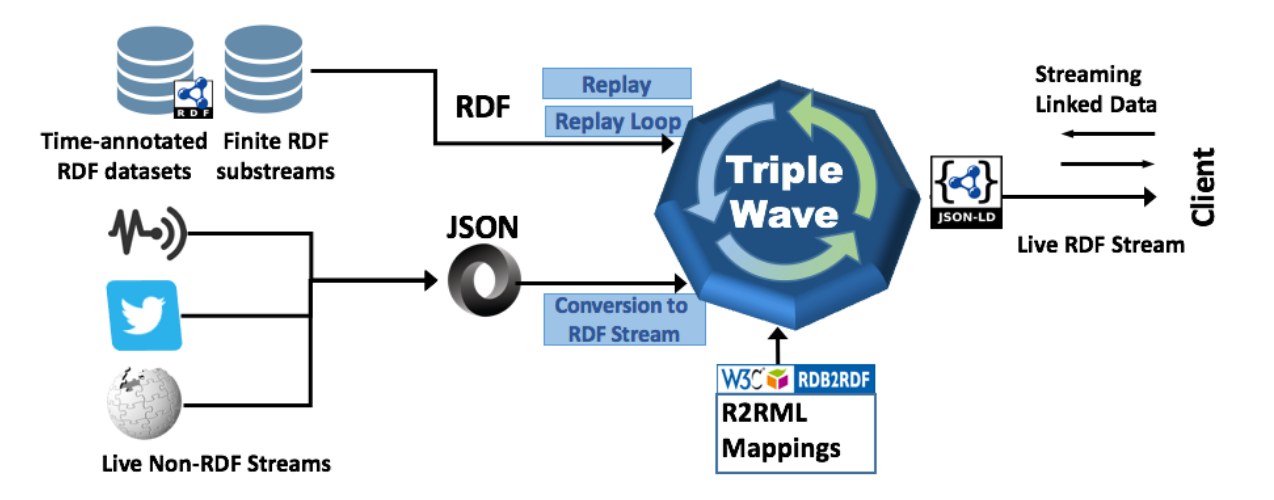
\includegraphics[width=\textwidth]{fig/triple-wave-arch.png}
  \caption{Architecture of TripleWave generating RDF streams from non-RDF and RDF data sources~\cite{triple_wave}. }
  \label{fig:triple-wave-arch}
\end{figure}

\subsection{RMLStreamer}
\label{sec:rml_streamer}
The engines elaborated thus far, scale insufficiently in terms of velocity and 
volume of data streams. Multiple instances of the engines will need to 
be started in order to scale with the higher volume and velocity of 
the input data streams. Since they are not built upon a distributed framework, 
there is also a need for a separate implementation to coordinate the different 
instances in a distributed environment. 

To tackle the aforementioned shortcomings, RMLStreamer~\cite{rml_streamer}
was developed to parallelize the ingestion and mapping process of RDF data generation pipeline. 
It is based on the work of RMLMapper~\cite{rml}, an RDF mapping engine consuming bounded data and 
mapping them to RDF data with the use of RML. Hence, RMLStreamer can also 
process heterogeneous data and generate RDF data. 

Due to the parallelization of the subtasks, the ingestion and the mapping process, these processes
could be spread over different machines for distributed execution. 
This is visualised in 
Figure \ref{fig:rml-parallel-arch}.  However, as with all distributed 
computing, a mechanism to coordinate the different machines is required. 
To fulfill this requirement, RMLStreamer is 
implemented on top of Apache Flink~\cite{flink} framework, a generic distributed stream 
processing framework. Not only does it allow the mapping 
of non-RDF to RDF data, it also guarantees fault-tolerance through the usage of 
\emph{Asynchronous Barrier Snapshots}~\cite{flink_fault_tolerance} and \emph{exactly-once} semantic,
although these are disabled by default. 

\begin{figure}[!htbp]
  \centering
  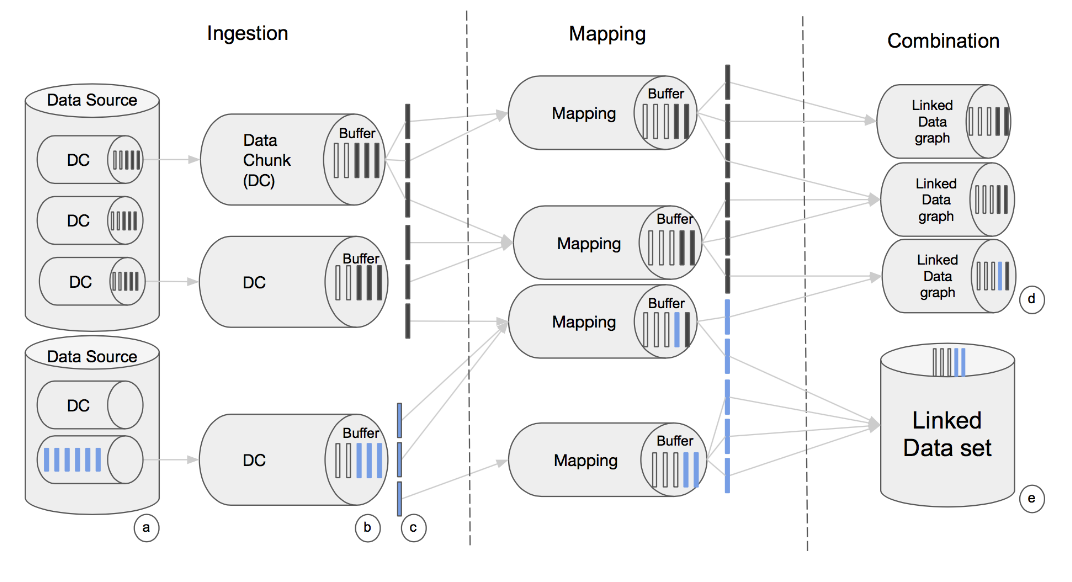
\includegraphics[width=\textwidth]{fig/rml_streamer_arch.png}
  \caption{Parallelization architecture of RMLStreamer for RDF data generation~\cite{rml_streamer}. RMLStreamer parallelizes 
  the ingestion of the data sources and the mapping process of non-RDF to RDF data. }
  \label{fig:rml-parallel-arch}
\end{figure}


\section{Summary}
While SPARQL-Generate~\cite{sparql_generate}, RDF-Gen~\cite{rdf_gen}, and TripleWave~\cite{triple_wave} 
support the join operator for executing a binary join, scalability is not built in those implementations
to handle multiple streaming 
data sources with high velocity and volume. 
Therefore, a solution
with built-in capabilities to handle high velocity and volume of data, is of interest
to implement the dynamic windowing scheme. 
Hence, RMLStreamer is the best candidate for this work on dynamic window in RDF generation. 

\chapter{Windows}
\label{chap:windows}

Due to the continuous, and infinite characteristics of streaming data, 
it is impossible to process the whole data in memory. Therefore, 
stream processing engines utilizes a buffer to hold the most recent stream of 
records in memory. This buffer is often called \emph{windows}. Windows make it 
possible to apply streaming version of the traditional data processing operators such
as joins~\cite{grubjoin}, sorts and aggregations. 

The behaviour of the \emph{windows} are configured through the specification of \emph{policies}
based on different characteristics; \emph{count}, \emph{attribute-delta}, \emph{time}, and
\emph{punctuation}-based policies~\cite{generic_window_sem}. For this thesis, only 
\emph{time}-based policy is of interest, specifically with the notion of \emph{event time},
since we are dealing with stream data with 
timeliness. Moreover, the definitions of the policies will be based on the 
implementations in Apache Flink and will differ from those defined by 
Bugra Gedit~\cite{generic_window_sem}. 


To understand the different \emph{windows} and \emph{policies}, we will elaborate them 
in the following sections. First, a few basic notations will be defined to 
help in the description of the semantic behaviour of the different 
\emph{windows} and \emph{policies}. Second, we will describe the mechanism of the 
different windows \textbf{with the semantic implication} imposed by the 
\emph{time}-based \emph{eviction}, and \emph{trigger} policies. 
Finally, a review of the different state-of-the art custom window operations 
will be discussed to aid us in the development of our methodology for 
the dynamic window processing. 


\section{Window Preliminaries}%
\label{sec:window_notations}

Before moving on to the discussion of the different \emph{windows}, we will introduce a 
few definitions and notations to describe the \emph{windows}. These notations and definitions 
will be used to aid in explaining the different semantic behaviour of the \emph{windows} under 
different \emph{policies}. 

\paragraph{Notations}%
$W = \{r_i | i \in [0\dots|W| - 1] \} $ is a window, whose size is denoted by $|W|$ in terms 
of the number of records inside the window $W$, and $r_i$ as the $i$th record inside 
the window. The records $r_i$'s are orderd from the newest to the oldest starting from 
$0\dots n$ with the oldest record being $r_n$ with $ n = |W| - 1$. The current record to be put 
into the window is denoted as $r_c$. The event timestamp associated with the
record $r_i$ is denoted as $\tau(r_i)$.

\section{Window Types}

According to Bugra Gedik~\cite{generic_window_sem}, windows could be categorized into 
three different types; \emph{tumbling} windows, 
\emph{sliding} windows~\cite{stream_standford,spade_stream}, and \emph{partitioned} windows.

\emph{Tumbling} and \emph{sliding} windows are also commonly provided as 
the default windows by the stream processing engines. 
They offer the most flexibility in customization with \emph{windows parameters} to fit 
most of the use cases.
\emph{Partitioned} windows are special variations of the \emph{tumbling} and
\emph{sliding} windows, where a partitioned window consists of different sub-windows of same size. 
This enables \emph{multiplexed processing} where independent computations are done across the 
different sub-windows at the same time, resulting in a higher throughput due to 
the parallelization of the processing~\cite{generic_window_sem}.

\subsection{Tumbling Window}%
\label{sec:Tumbling Window}
Tumbling windows have a \emph{fixed} window size and do not 
overlap. The size of the window influences 
the number of elements residing in the window. It stores the elements 
until the window is \emph{full} and this is determined by the \emph{eviction} policy. 
In the context of this thesis, the \emph{size} of the window will be defined by 
a time period bounded by a lower and a higher event timestamp. 

Processing of the elements within the window happens only when a \emph{trigger}
event is fired. This is determined by the \emph{trigger} policy which fires the 
\emph{trigger} event. For tumbling windows, the default \emph{trigger} policy is 
fulfilled when the window is \emph{full}.


\paragraph{Eviction}%
Extending the notations used in Section~\ref{sec:window_notations}, we define 
the even-time-based tumbling window $W = \{r_t |  t \in \tau(r_0) \dots \tau(r_n) \}$. 
Then, the size of the window is $|W| = [\tau(r_l), \tau(r_h)[$, where the 
$\tau(r_l)$ and $\tau(r_h)$ represents the lower and the upper bound of the 
records timestamp respectively. 
Current record $r_c$ must therefore, have a timestamp  $\tau(r_l) \le \tau(r_c) \le \tau(r_h)$ 
to be accepted by the window. If $\tau(r_c) \ge \tau(r_h)$, the record will be 
considered late as described in watermarking mechanism in Section~\ref{sub:Out of order processing}. 


Since tumbling windows are processed only when the window is \emph{full}, \emph{trigger} events 
are fired at the same time as \emph{eviction} events for tumbling windows.


\subsection{Sliding Window}%
\label{sec:Sliding Window}
Similar to tumbling windows, sliding windows also have \emph{fixed} window size 
that is immutable throughout the lifetime of a stream processing engine. 
In addition to the window size as a parameter, one could also specify the 
\emph{window slide} for sliding window. This parameter specifies how frequently 
a sliding window is created. 
Therefore, if the \emph{window slide} is smaller 
than the \emph{size} of the window, an overlap will be formed and multiple 
windows could exists at that point of time. The records in the overlapped region 
will have to be copied across the multiple overlapping windows. 
Taking the \emph{slide} and the \emph{size} into account, we could conclude that 
tumbling window is a special case of sliding window where the \emph{slide} is 
equal to the \emph{size} of the window.

Due to the overlapping of the windows, extra checks has to be considered 
when evicting the elements in the sliding windows, to ensure that the elements in 
overlapping windows are not removed from the multiple windows. To overcome this overhead 
of checking when evicting the window, 
stream processing engines copies the records across the overlapping windows. 
This is a trade-off of processing time to keep the latency low for higher memory consumption. 

The \textbf{two \emph{policies}} for the sliding windows are the same as those for the \emph{tumbling} windows. 

\begin{figure}[htpb]
    \centering
    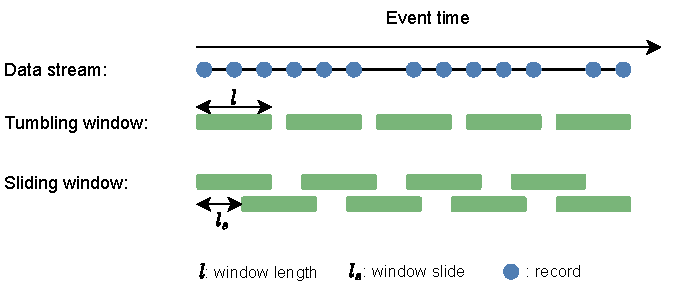
\includegraphics[width=0.8\linewidth]{fig/slide_tumb_windows.pdf}
    \caption{Sliding and tumbling window applied on a data stream~\cite{jonas_scotty}. }%
    \label{fig:slide_tumb_window}
\end{figure}


\subsection{Partitioned Window}%
\label{sec:Partitioned Window}

Unlike the aforementioned types of window, where windowing is applied on the stream 
without any changes to the stream, partitioned windows split the data stream into 
different substream based on the \emph{key} of the partition. This enables the 
techniques of \emph{multiplexed processing} to be applied on the data stream, increasing 
the parallelization of stream processing engines. 

\paragraph{Multiplexed processing}%
\label{par:Multiplexed processing}
Most data stream could be split up into multiple substreams consisting of records 
of the same \emph{key} attributes. This is akin to 
the \emph{groupBy} operations present in the traditional batch data processing where 
data records are grouped according to a specific set of the records' \emph{attributes}.
For example, consider a stream containing 
Twitter tweets~\footnote{Twitter API: \href{https://developer.twitter.com/en/docs/twitter-api/v1/data-dictionary/object-model/tweet}
{Twitter's tweet object model documentation.}}. These stream \emph{tweets} could be 
partitioned into substream based on the user's id. 
Therefore, to support multiplex processing, any operators applied on the substreams 
must be local to that particular substream. The operators also need to keep the states for each 
substream independently. 


Partitioned windows support \emph{multiplexed processing}, since it consists of  
multiple subwindows; each corresponding to a particular substream identified 
by the \emph{key} attribute of the records in the data stream. The subwindows 
are independent from each other and all computations on the records are in the local scope 
of the subwindow. The actual subwindow semantics can be of the aforementioned types 
of windows; \emph{tumbling windows} or \emph{sliding windows}. Therefore, the 
\emph{eviction} and \emph{trigger} policies of the subwindows 
are similar to those two types of windows. 


\begin{figure}[htpb]
    \centering
    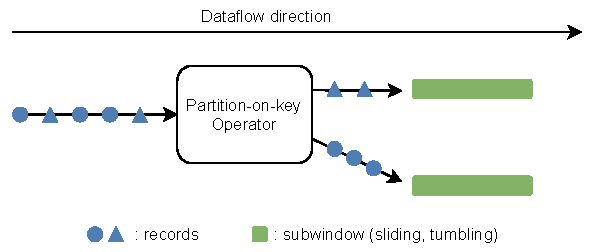
\includegraphics[width=0.8\linewidth]{fig/partitioned_window.pdf}
    \caption{Partitioned window where the records are keyed by an attribute. In this case,
    records are keyed by their shape. After \emph{keying} the records, circle records are sent 
    to a subwindow different from the triangle records.}%
    \label{fig:partitioned_window}
\end{figure}
   

\section{Windows processing}
\label{sec:windows_processing}

Streaming applications requires some form of queries to be executed over 
the data stream. Joins and aggregations are some of the most common queries 
in stream processing which we will elaborate in the upcoming sections. 

\subsection{Aggregation}%
\label{sub:Aggregation}
Window aggregations are a class of operations where some form of computations 
is done on a group of records within a window. Operations like 
finding the \emph{maximum value} or \emph{average value} are some of the 
aggregations frequently done in data stream processing. However, 
aggregate operations can be expensive in some situations. 
For example, aggregations operations are expensive when there is 
an overlap of windows (sliding windows), since aggregations over the overlapping 
records will need to be recomputed for each overlapping windows. Given a sliding 
window of 1 minute \emph{size} and 1 seconds \emph{slide}, 60 windows will exist 
at any point of time and the 59 seconds worth of records aggregation will need 
to be recomputed whenever a window receives a \emph{trigger} event for processing. 
This results in redundant computation. 

Sufficient amount of studies have went into optimizing the aggregation queries 
on windows. Jonas et al~\cite{scotty, jonas_scotty} have come up with a method to 
apply generic window \emph{slicing} for optimizing aggregation operators in windows. 
The data stream is modelled as \emph{slices}, where 
records are assigned to exactly one \emph{slice} resulting in a 
$O(1)$ complexity for memory. The \emph{slices} are created every time a 
window begins or ends. Partial aggregations are then applied on the 
records within the slices which will eventually be consolidated once 
a window ends for a final aggregation result eliminating redundant 
computations. According to the authors~\cite{jonas_scotty}, this maintains 
the high throughput processing capabilities of Apache Flink even if the 
number of overlapping concurrent windows increases. 


\subsection{Join}%
\label{sub:Join}

Join operations are different from that of aggregations. We do not need 
to wait for the window to be full, before processing the records inside the 
window. A \emph{trigger} event could be fired at the very moment a new 
record arrives in the window. Several studies have been conducted    

\chapter{Methodology}%
\label{chap:Methodology}


In this chapter, we introduce an approach to dynamic windowing 
in data stream processing 
with the following improvements to fixed size windows; 
\begin{enumerate*}[label=(\alph*)]
    \item stream-characteristic-aware processing 
    \item adaptive window sizes, and 
    \item high throughput with low latency processing. 
\end{enumerate*}

Existing fixed size windows are inflexible when the characteristics of a data stream,  
such as the stream rate, change over time. Either the window size is 
too small to produce any output or too large which leads to high memory usage when 
the stream rate is high. Furthermore, fixed size windows only process the 
records inside the window at fixed interval (usually equal to the size of the window). 
This leads to high latency proportional to the window size. As a consequence, 
it causes unnecessarily high latency in some operations, where records could be processed once it arrives inside 
the window. One example of such operation is the join operator, where the joined 
result could be emitted the moment a new record arrives inside the window. 
Solving these disadvantages leads us to our approach 
of a dynamic window, which can adjust its size during runtime,
resulting in a low latency and high throughput solution. 


This chapter will be outlined as follows. 
First, we analyse the possible sites across the different stages of 
RMLStreamer to implement our dynamic window. Next, we define which operator
(join, aggregation, etc \dots) to implement as the reference processing operator inside 
our dynamic window. Subsequently, we elaborate our dynamic window algorithm to allow 
dynamic adjustment of window sizes depending on the stream rate of the incoming records.  
Finally, we give a brief overview of our reference implementation.



\section{Analysis for the implementation site}
\label{sec:analysis implementation site}
There are two possible sites to implement our dynamic window; 
\emph{before} or \emph{after} the mapping of non-RDF to RDF data. There are different trade-offs for choosing one 
over the other. 

\paragraph{After the mapping process}%
Implementing the windowing operations after the mapping process allows the 
possibility of applying graph processing operators in the window; the input data for 
the windows will be RDF triples from the mapping process. 

However, it comes with a major disadvantage. All the attributes required in the operator 
will have to be mapped in the mapping stage to their corresponding triple statements. 
This could lead to an explosion in the number of triple statements being generated, increasing 
the network cost of sending the data to the windowing stage. High latency processing in 
the mapping stage will also occur if the amount of attributes required by 
the operator is sufficiently large enough. 


\paragraph{Before the mapping process}%
\label{par:Before the mapping process}
To mitigate the explosion of triple statements after the mapping process, we could implement 
the windowing right before the mapping process. A reduction in the amount of 
data needed to be processed in the mapping stage could be achieved by operators 
such as \emph{filter} or \emph{joins} in the windowing stage. Furthermore, direct 
access to the raw data allows more arbitrary transformations to be applied such as 
those specified in FnO~\cite{fno_ben}, without the loss of 
information due to mapping process. 

If graph processing operations are required, we could delegate the processing computations to 
existing state-of-the-art RDF stream processing engines by attaching them at the output of 
RMLStreamer. In conclusion, it is ideal to implement the windowing before the mapping process. 


\begin{figure}[htpb]
    \centering
    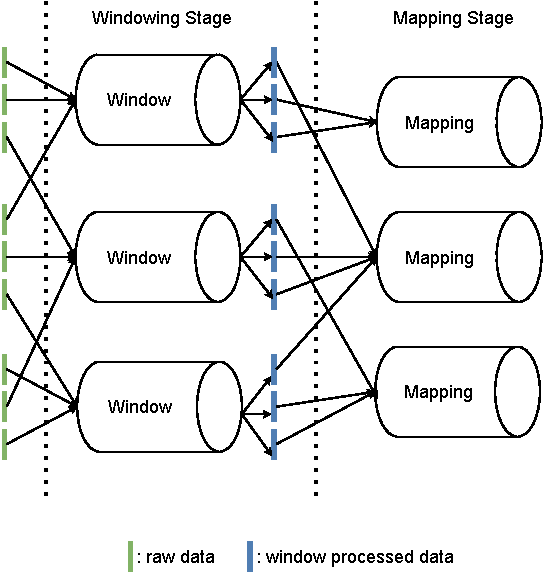
\includegraphics[width=0.7\linewidth]{fig/window_site.pdf}
    \caption{Implementation of windowing stage \textbf{before} the mapping stage. The blue blocks 
    are chunks of processed records of an \emph{operator} (join, aggregation, etc\dots) in the windows. 
    The green blocks are raw data chunks from the 
    ingestion stage (Figure~\ref{fig:rml-parallel-arch}). }%
    \label{fig:fig/s}
\end{figure}


\section{Operator inside window}
\label{sec:Operator inside window}
Which type of operation is suitable for our dynamic window? 
In the context of this work with RMLStreamer, we will have to consider optimizing the 
\emph{join} operation.

RDF mapping engines focus 
on just mapping the input to RDF compliant formats without 
applying complex stream processing queries like \emph{aggregations} and 
\emph{reductions}. These stream processing queries, if required, could be 
delegated to RDF stream processing frameworks processing RDF data streams.
Therefore, we focus on a reference implementation of dynamic windows with 
stream joins as part of the mapping process of heterogeneous data streams 
to RDF data streams.




\section{Dynamic Window}%z
\label{sec:Dynamic Window}
A dynamic window is a type of partitioned window (Chapter~\ref{sec:Partitioned Window}).
We define it as a group of subwindows, which update their sizes dynamically according to the characteristics 
of the data stream. It groups the incoming streams into different partitions first, according to 
the \emph{key} attribute value of the records. Subsequently, these grouped records are assigned 
to individual subwindows. These subwindows adjust their own size independently from each other 
at each update cycle. Furthermore, the subwindows will be independent from each other such 
that the stream rate is local to the attribute value for which each subwindow is responsible. 

We shall first extend the notations in Chapter~\ref{sec:window_notations} to aid in the 
elaboration of our dynamic window. Finally, the full algorithm for dynamic windowing 
is described in detail in pseudo code. 


\paragraph{Notations}

Similar to the notations in Chapter~\ref{sec:window_notations}, we extend the 
notations used in~\cite{generic_window_sem}. 
$W^{a} = \{ W^{a=v} | v \in \{r.a | r \text{ is a record in } W^a\}\}$ is a dynamic window, 
where $a$ represents a \emph{key} attribute. $|W^a|$ is the number of subwindows 
in $W^a$, and $W^{a=v}$ represents a subwindow associated with a \emph{key} attribute value 
$v$. Each subwindow is defined as $W^{a=v} = \{r_{i}^{a=v} | i \in [0\dots|W^{a=v}|-1]\}$, 
where $r_{i}^{a=v}$ are ordered from the newest to the oldest starting from 
$0\dots n$ with the oldest record being $r_{n}^{a=v}$ with $n = |W^{a=v}|-1$. 
The current record to be put into the subwindow $W^{a=v}$ is denoted as $r_{c}^{a=v}$. 
The \textbf{event} timestamp associated with the record $r_{i}^{a=v}$ is denoted as 
$\tau(r_{i}^{a=v})$. 

The two streams to be joined are denoted as $S_P$ and $S_C$, for 
streams representing the parent triple map and child triple map respectively~\cite{rml}. 
The number of records in the subwindow $W^{a=v}$ from $S_P$, and $S_C$ are respectively 
denoted as $|S_{P}^{a=v}|$, and $|S_{C}^{a=v}|$. The list states, 
a data structure to hold the records from $S_P^{a=v}$ and $S_C^{a=v}$, 
are respectively denoted as $List_P^{a=v}$ and $List_C^{a=v}$. 
We also denote the 
pseudo maximum size of the list states  $List_P^{a=v}$ and $List_C^{a=v}$
as $Size(List_P^{a=v})$ and $Size(List_C^{a=v})$ respectively. A record from $S_P^{a=v}$ or $S_C^{a=v}$  
is denoted as $r_i^{a=v,P}$ or $r_i^{a=v, C}$ respectively.

We also define a threshold $\epsilon$ used to check if the window size needs 
to be adjusted based on the join cost $m$. Generally, if $\epsilon = 1.5$, it represents 
the threshold where the number of records inside a subwindow, $W^{a=v}$, 
is $1.5$ times the size of $Size(List_P^{a=v}) + Size(List_C^{a=v})$.  

\subsection{Dynamic window join}
\label{sub:Dynamic window join}

The join algorithm used, is a variant of Symmetric Hash Join~\cite{symmetric_hash_join}. 
The subwindow themselves work like a hash table, containing records with a 
specific \emph{key} --- since they are \emph{partitioned} (Chapter~\ref{sec:Partitioned Window}). 
The records are joined by probing the relevant stream and generating the 
joined result. 

We will work through a simple example when a record $r_c$ arrives 
inside a subwindow $W^{a=v}$. For ease of writing, we omit $a=v$ in our notations. 


\begin{exmp}    
    Provided the incoming record is $r_c^{P}$, we first insert 
    it into $List_P$. Subsequently, we probe for 
    $\forall i, r_i^C \in List_C$, and join all $r_i^C$ found, with $r_c^P$
    as tuples of $(r_c^P, r_i^C) \text{ with } \forall i, r_i \in List_C$.
    Similar steps are executed for $r_c^C$. 
\end{exmp}





\subsection{Dynamic window sizing}%
\label{sub:Dynamic window sizing}
For each subwindow $W^{a=v}$, the following configuration parameters 
are provided: 

\begin{itemize}
    \item $\Delta n$: the \textbf{initial} interval of time before the next eviction trigger (Chapter \ref{chap:windows}). 
    \item $\epsilon_u$: the upper limit for threshold $\epsilon$.
    \item $\epsilon_l$: the lower limit for threshold $\epsilon$. 
    \item $U$: the upper limit for the window size. 
    \item $L$: the lower limit for the window size. 
\end{itemize}



For ease of writing, we will omit $a=v$ to specify the \emph{key} attribute associated 
with the subwindow. 
Therefore, the following events happen for every subwindow $W^{a=v}$ independently from 
each other. 

Since we are implementing the join operator, the trigger event is fired when  
$r_c$ arrives, and the join operation in Chapter~\ref{sub:Dynamic window join} is 
executed. 


The eviction trigger is fired every time when the current watermark (Section \ref{ssub:Watermarking}) 
$w \ge |W| + \Delta n$. At each eviction trigger we calculate the 
the cost for each \emph{list states} $List_P$ and $List_C$, containing the records from $S_P$ and $S_C$
respectively. The cost for $cost(List_P) = |S_P|/Size(List_P)$, idem for $cost(List_C)$. 
The total cost is $m = cost(List_P) + cost(List_C)$ and it is checked against thresholds $\epsilon_l$ and $\epsilon_u$. If  $\epsilon_l \le m \le \epsilon_u$, 
$\Delta n$ stays the same, otherwise it will be adjusted accordingly. This provides some stability 
in window sizing by keeping the same size, if the cost lies within the thresholds. 
The higher $m$, the higher the stream rate. Thus, the subwindow needs to be frequently 
evicted and lower $\Delta n$ to reduce memory usage. There is also a limit on the 
minimum and maximum window sizes, $L$ and $U$ respectively, to ensure that the window 
size $\Delta n$ does not keep growing or shrinking in size infinitely, in worst case scenario. 
The sizes of the list states 
are also updated according to $Size(List_P) = Size(List_P) * cost(List_P) + 0.5$.
Similarly for $Size(List_C)$. 
Hence the dynamic window maintains an 
ideal size by adjusting $\Delta n, Size(List_P)$ and $Size(List_C)$ according to 
the stream rate. The pseudo code for the eviction algorithm is presented in Algorithm~\ref{alg:dynamic_eviction}.

This algorithm for the dynamic window is an adaptation of the VC-TWindow~\cite{vctw_join} with 
improvements for stability in window sizing, clarity in the metrics used for updates, and localization 
of window size update to each subwindow.  

\begin{algorithm}[htbp]
    \DontPrintSemicolon
    \KwData{$\Delta n, \epsilon_u, \epsilon_l, U, L, List_P, List_C, S_P, S_C$}

    \tcp{Note: cost(..) is ratio for how "full" a list-state is} 
    $cost(List_P) = |S_P| / Size(List_P)$      \tcp*{Calculate the cost (ratio) of list-state P } 
    $cost(List_C) = |S_C| / Size(List_C)$      \tcp*{Calculate the cost (ratio) of list-state C } 


    total cost $ m = cost(List_P) + cost(List_C)$  
  
    \If{$m > \epsilon_u$} 
    {
        \tcp{the cost is too high, shrink the window size and adjust list-states}
        $\Delta n = \Delta n / 2 $ 
        
        $Size(List_P) = Size(List_P) * (cost(List_P) + 0.5)$  

        $Size(List_C) = Size(List_C) * (cost(List_C) + 0.5)$  
    }
    \ElseIf{$m < \epsilon_l$}
    {
        \tcp{the cost is too low, increase the window size and adjust list-states}
        $\Delta n = \Delta n * 2$ 

        $Size(List_P) = Size(List_P) * (cost(List_P) + 0.5)$  

        $Size(List_C) = Size(List_C) * (cost(List_C) + 0.5)$  
    }

    clean both $List_C \text{ and } List_P$
    \caption{Dynamic window $onEviction$ routine}
    \label{alg:dynamic_eviction}
\end{algorithm}



\section{Implementation}%
\label{sec:Implementation}

The dynamic window is implemented for RMLStreamer 
to extend its capabilities to do simple stream processing by 
joining multiple streams. RMLStreamer is implemented in Scala 
on top of the Apache Flink framework and with Flink's easy to access, low-level APIs, 
we could easily implement our custom dynamic window.  

Furthermore, new \emph{properties} and \emph{classes} are defined to extend RML with 
support for window configurations. RML's extensibility allows us to 
define new RML vocabularies without changing the existing ones. The ontology 
definitions is rudimentary at this moment and it is used only to configure our 
window type. However, it could easily be extended to also include windo specific 
parameter configurations if required. An example of this RML mapping file for 
dynamic window can 
be found in Appendix~\ref{lst:dynamic_mapping_file}. For example, one could 
adjust the window type by changing the literal value for the property 
\emph{rmls:windowType} with either \emph{rmls:Tumbling} or \emph{rmls:DynamicWindow}. 








 





\chapter{Evaluation}
\label{chap:Evaluation}

To measure the effectiveness of dynamic windowing for multi-stream operators during the 
mapping of non-RDF heterogeneous data, we would need to measure the following 
metrics of our stream processing framework: \emph{latency}, \emph{throughput},
\emph{memory usage} and \emph{completeness}. \emph{Throughput}, in this 
paper, refers to the number of processed input records, per time unit.
\emph{Latency, throughput,} and \emph{memory usage} can be measured following the recent benchmark studies by 
Van Dongen and Van den Poel(2020)~\cite{evalution_of_spe}.
However, to evaluate 
for the \emph{completeness}
of the generated output, a reference output needs 
to be generated for comparison. Since a data stream is unbounded in nature, 
and cannot be processed completely to check for \emph{completeness}, a bounded 
dataset of relatively large volume will be used to measure \emph{completeness}.
To ensure consistency in the complexity of the multi-stream operator being used, 
we will apply the join operator in the windows --- a common operator used in 
data enrichment scenarios. 

The following sections will describe the methodology and the data used to evaluate the
different metrics. Setups required to reproduce the evaluation will also be elaborated 
in their respective sections. 


\section{Data}

Assessment of our dynamic windowing scheme for multi-stream operator will require 
the data to have some common attributes to enrich the data. Furthermore, to 
mirror a real-world scenario, we would also employ data gathered from IoT sensors. 
We will use the same data 
as the benchmark in the paper by Van Dongen and Van den Poel~\cite{evalution_of_spe}. 
The data is provided by NDW (Nationale Databank Wegverkeersgegevens) from the 
Netherlands~\footnote{NDW data site: \href{http://opendata.ndw.nu/}{http://opendata.ndw.nu/} }.
It consists of measurements of the number of cars and their average speed across  
A subset of the complete sensor data will be replayed by a Kafka publisher into the two topics 
\emph{flow} and \emph{speed}, for the number of cars and the average speed respectively. 

\subsection{Data for completeness evaluation}
Evaluating completeness requires a dataset which could be mapped completely by a static 
mapping engine. 
Our \emph{complete} set of output triples will be generated according 
to the RML mappings. Streaming data is usually 
ordered according to the event time (Chapter~\ref{chap:data_stream_processing}) 
and the same entity could appear in the 
stream at a different timestamp. This can lead to duplicates in the generated output by 
the bounded data processing by RMLStreamer. Duplicates, in this context, are triples that semantically describe the 
same knowledge. Therefore, duplicates in the generated output by the reference optimal
mapping engine needs to be removed in the final \emph{complete} output dataset.

\section{Evaluation pipeline}

\begin{figure}[!htbp]
    \centering
    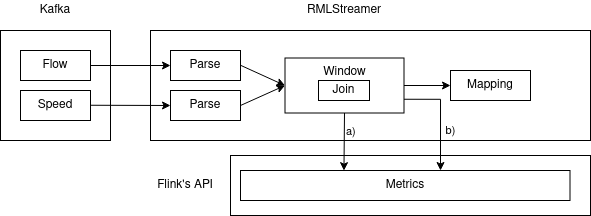
\includegraphics[width=\textwidth]{fig/evaluation_architecture.png}
    \caption{Evaluation flow based on~\cite{evalution_of_spe} with some changes to only 
    take metrics at the "Join" stage.
    a) \emph{latency, memory}, and \emph{cpu usage} of evaluating the join operator in windows.
    b) \emph{throughput} of the generated output triple.}
    \label{fig:evaluation_flow}
    
\end{figure}

Similar to the workflow process in~\cite{evalution_of_spe, benchmark_sce}, we set up
our evaluation pipeline as illustrated in Figure~\ref{fig:evaluation_flow}. Setting it 
up according to the illustrated pipeline, allows us to have fine control over the 
workload scenarios and limit the measurement of the metrics just to the windows. 




\section{Workload scenarios}
Data streams have characteristics 
which determine the performance of stream processing frameworks and its 
operators (Chapter~\ref{chap:data_stream_processing}). Therefore, 
there is a need to evaluate our dynamic window implementation under different workload scenarios. 

\subsection{Workload for maximum throughput measurement}
This workload will measure the maximum throughput RMLStreamer can 
process with the different windows, before \emph{latency,} and \emph{memory utilization}
increase significantly~\cite{benchmark_dsdps}. We will increase the velocity of the input data gradually 
every 10 seconds until there is a significant latency of more than 10 seconds to produce
the next output triple or until the memory allocated to the instances get fully used up. 


\subsection{Workload for latency measurement}
As described in the paper by Van Dongen and Van den Poel~\cite{evalution_of_spe}, 
\emph{throughput} and \emph{latency} can affect each other if the workload is 
improperly configured. Therefore, measurement of the \emph{latency} caused only 
by the window implementations, requires the stream processing framework to not be 
stressed under significant \emph{throughput}. Thus, the Kafka broker will 
publish the records at a very low constant rate of around 200 messages per second. 

Since \emph{latency} is also measured with a time unit, the timestamp of the 
records are important for \emph{latency} measurement. Due to the replay of the dataset 
through the Kafka broker, it is imperative to use the local timestamp of the same Kafka broker
attached to the input and output records for \emph{latency} 
measurement\cite{latency_measurement_kafka}.
\gh{Maybe you can tune Kafka to keep its latency as low as possible, so that the timestamps of the (Kafka) messages don't deviate too much from the event time stamps. If you do, you also have to describe that in the set-up}


\subsection{Workload for completeness}
The implementation of the dynamic window should also ensure that the generated 
output is as \emph{complete} as possible. The bounded dataset will be processed fully by 
a reference mapping engine. The generated RDF graph by the reference 
engine will be \emph{complete}. It will be used to compare with the result 
generated by the RMLStreamer for each window being evaluated. 

Depending on the type of window being used, \emph{completeness} of the output will be
affected by the window size. If the window size is not sufficiently large enough to handle 
the input velocity, the next incoming record will be processed in the new window instead of 
the old window where it is more relevant to the other records in the old window. Thus, 
we will vary the stream rate to measure the \emph{completeness} of the results generated 
with the use of different windows.

\subsection{Workload with periodic burst}
Fluctuation in the streaming sources are normal with unstable network connections. 
The windowing operator must therefore be able to cope with sudden changes in the 
fluctuation of the velocity of the data stream. This workload attempts to emulate 
the scenario where multiple IoT devices sends data in bursts with a periodic 
time interval. The workload will have a constant low stream rate with occasional 
bursts of data every few seconds. 


\section{Environment}

RMLStreamer will be evaluated in a virtual environment provided imec IDLabt from Ghent 
University called Virtual Wall\footnote{Virtual Wall: \href{https://doc.ilabt.imec.be/ilabt/virtualwall/index.html}{https://doc.ilabt.imec.be/ilabt/virtualwall/index.html}}.
Virtual Wall provides us with machines to run our tests remotely with consistent 
hardware specifications. It also provides the developers with the ability to induce 
artificial network impairment such as delay, packet loss, and bandwidth limitation. Such 
flexibility in the configuration allow us to devise a scenario as close to a real-world use case. 

For this work, we will be making use of it to set up the testing 
environment and mimic it as closely as possible to a real-world scenario. 
To prevent the publishing of data from taking up the resources used for evaluating the 
window operators, a Kafka broker will be run on a separate node. RMLStreamer will then be 
executed on a standalone node. Only a single Kafka broker will be used throughout the experiment, 
to ensure that the \emph{latency} measurement all comes from the same wall clock of the machine. 
Different Kafka brokers could be used in the experiment and then synchronized again 
with Network Time Protocol (NTP). However, the latency will still have a minimum
error of 35 ms~\cite{ntp_latency} \gh{Is this still valid today? Also, the clocks of the nodes on the virtual wall are synced with high precision (have to check if we find a reference for this though)},
which is not suitable to measure the sub 10ms latencies in 
real-time applications. Therefore, we opted to use only a single Kafka broker to publish
our data stream for evaluation.






\chapter{Results}%
\label{chap:Results}

In this chapter, the results gathered from our evaluation of the dynamic window against 
the tumbling window will be discussed by the order of the workloads. The workload 
evaluations are run multiple times for consistency of results. We will first 
discuss the workload for latency measurement, followed by periodic workload and 
finally the completeness measurement. For each workload results, we elaborate 
and discuss in details the shortcomings of the evaluation methods and the 
possible outlier situations for which the evaluation result would not agree with.



\section{Workload for latency measurement}%
\label{sec:Results Workload for latency measurement}

This workload is run with a constant low stream rate to ensure that 
the RMLStreamer is not overloaded for a more accurate latency measurement. We also measured 
CPU, throughput, and relative memory usage to determine the improvement brought by Dynamic window
in an ideal streaming environment.

For latency, Tumbling window has a median value of 1915ms, with latency ranging from 1081ms to 2624ms. 
This is as expected since the window is measured using the \emph{average} latency of all records used 
in the joined result at every \emph{trigger} event, which is fired every 2 seconds (the size of tumbling window).
In contrast, Dynamic window has sub second latency with median 57ms and ranging from 39ms to 120ms. Clearly, 
our improvement to fire the \emph{trigger} event whenever a new record arrives inside the subwindow, allows 
Dynamic window to achieve sub second latency. 

Just like latency, the throughput difference between the two windows is also significant. Dynamic window has a 
steady throughput of around 17200 records per second whereas Tumbling window fluctuates around 
12500 and 12800 records per second before stabilizing at 12750 records per second. This is expected as Dynamic 
window eventually stabilizes to a window size with the capability of processing more records than Tumbling window. This is 
due to the adjustment of window sizes at the subwindow level, allowing Dynamic window to wait for more records 
with infrequent \emph{key} attribute in the stream, before evicting the subwindow. In contrast, Tumbling window 
always evicts the content of the window after 2 seconds, even if it means that there might be more 
eligible records to be joined with the records in the soon to be evicted window, leading to lower throughput.  

Relative memory usage of Dynamic window compared to Tumbling window is similar over the lifetime of the 
evaluation run (Figure~\ref{fig:constant_mem_diff}). Dynamic window causes infrequent \emph{spikes} in memory of more 
than 100 MB memory usage than Tumbling window at certain point in the lifetime of evaluation. This can be attributed 
to the subwindows of Dynamic window growing larger than Tumbling window due to not enough records of the same 
\emph{key} attributes arriving inside the subwindows. However, Dynamic window stabilizes to a more optimal 
window size, where it uses less memory than Tumbling windows, over longer stretches of the evaluation run. At worst case, 
it uses as much memory as Tumbling window does over the course of the evaluation. 

CPU usage is higher by around 7\% for Dynamic window since it requires extra processing of the calculation of metrics. However, this 
increase in CPU usage can also be attributed to the increase in throughput, where the RMLStreamer has more joined results 
to process and map to RDF data.  

\begin{figure*}
    \begin{subfigure}[b]{0.5\textwidth}
        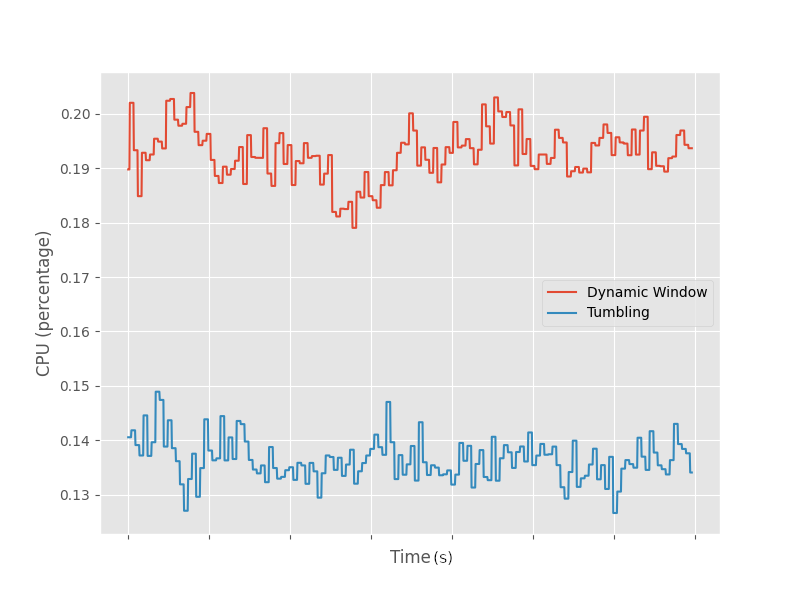
\includegraphics[width=\textwidth]{fig/constant-rate/cpu_comparison.png}
        \caption{CPU usage}
        \label{fig:constant_cpu}
    \end{subfigure}
    \hfill 
    \begin{subfigure}[b]{0.5\textwidth}
        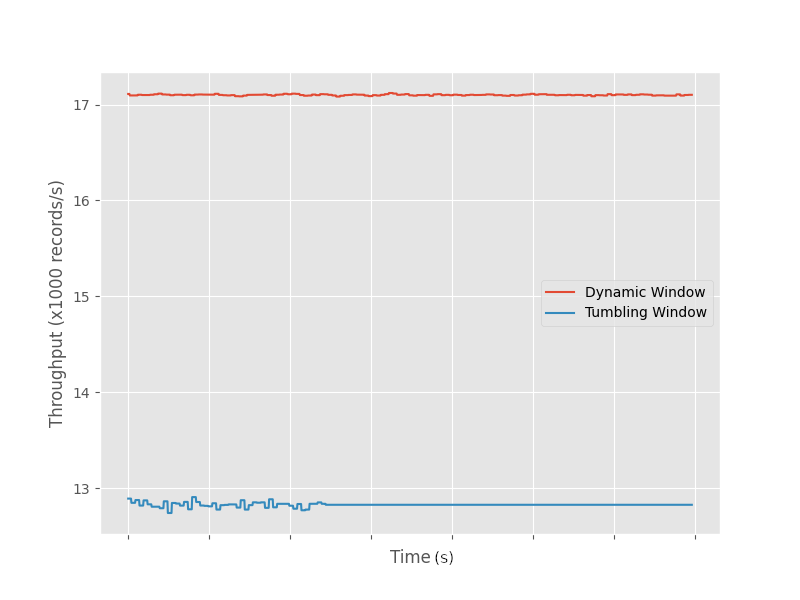
\includegraphics[width=\textwidth]{fig/constant-rate/throughput_comparison.png}
        \caption{Throughput of joined records}
        \label{fig:constant_thorughput}
    \end{subfigure}
    %%
    \begin{subfigure}[b]{0.5\textwidth}
        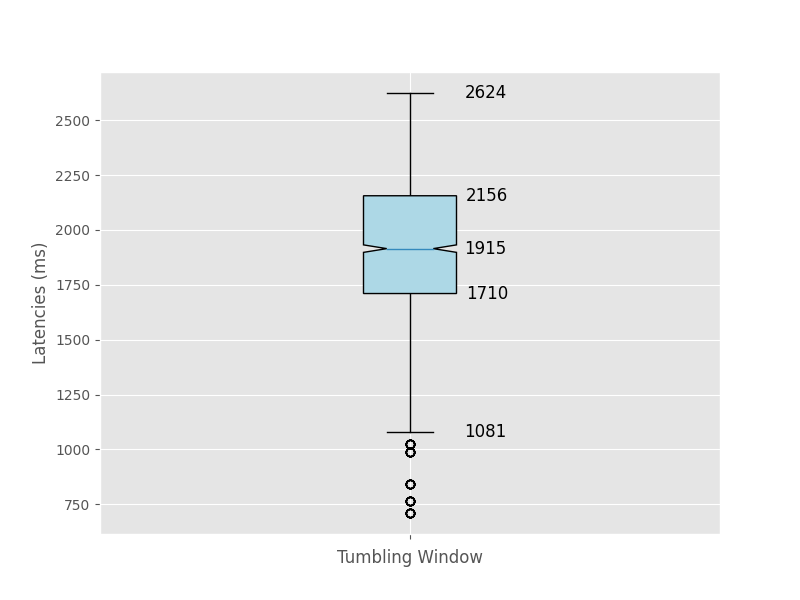
\includegraphics[width=\textwidth]{fig/constant-rate/TumblingWindow_latency_boxplot.png}
        \caption{Tumbling latency}
        \label{fig:constant_tumb_boxplot}
    \end{subfigure}
    \hfill 
    \begin{subfigure}[b]{0.5\textwidth}
        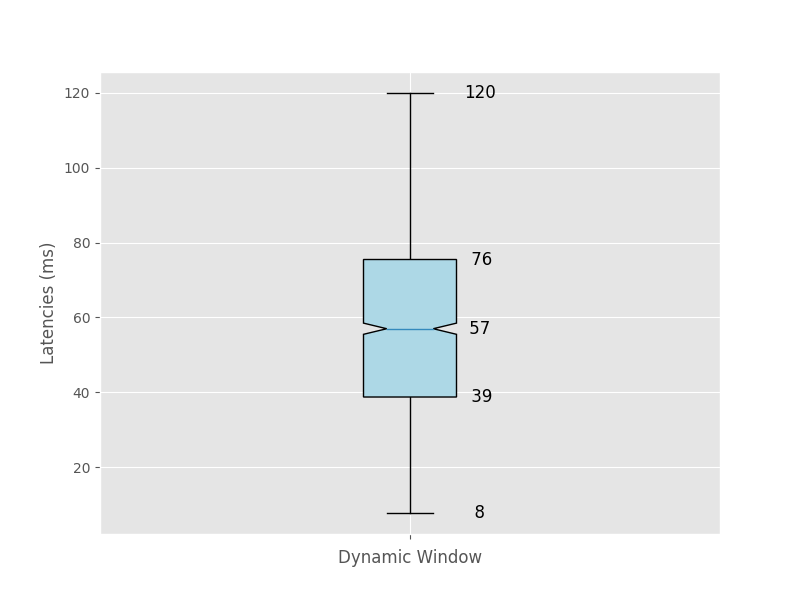
\includegraphics[width=\textwidth]{fig/constant-rate/DynamicWindow_latency_boxplot.png}
        \caption{Dynamic latency}
        \label{fig:constant_dynamic_boxplot}
    \end{subfigure}
    % 
    \begin{subfigure}[b]{\textwidth}
        \centering
        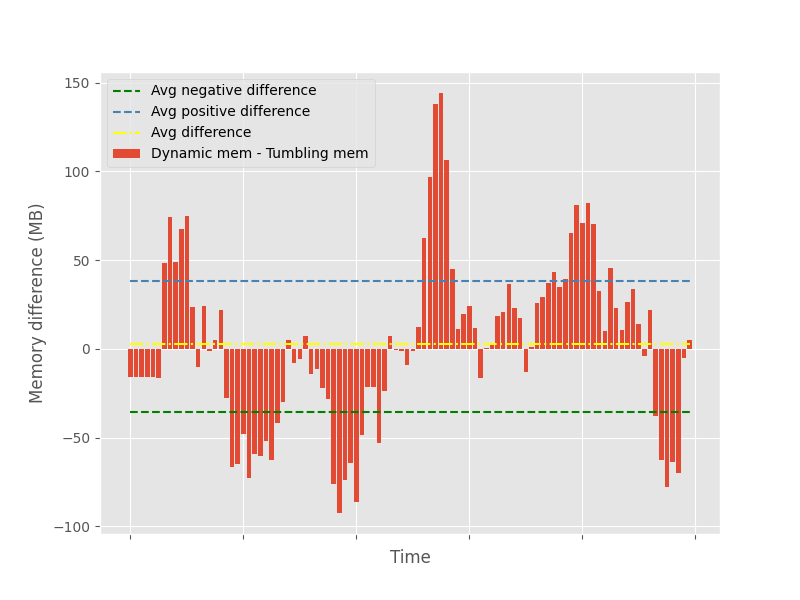
\includegraphics[width=0.5\textwidth]{fig/constant-rate/mem_difference_bar.png}
        \caption{Relative difference in memory usage from the perspective of dynamic window}
        \label{fig:constant_mem_diff}
    \end{subfigure}

    \caption{Metrics measurements for latency workload.}%
    \label{fig:constant_measurement}
\end{figure*}

\newpage
\section{Workload for periodic burst}%
\label{sec:Results Workload for periodic burst}

Dynamic window still handles the periodic burst of data with lower latency 
than Tumbling window with latency in the range from 8ms to 1669ms compared to 
Tumbling window's range from 891ms to 3904ms.
However, there is a temporary increase in latency at the beginning 
(Figure~\ref{fig:periodic_dynamic_lineplot}), 
when the burst of data arrives at every 10th second. 
This is due to the initial size of 2s subwindows for the initial low stream rate of 400 records per second. 
The subwindow sizes start to grow \textbf{larger} than 2s because of the low stream rate. 
The increase in the subwindow size results in the window 
window having more records to join; causing a back pressure to form and latency to increase.  
This results in a positive skew in the latency distribution for Dynamic window (Figure~\ref{fig:periodic_dynamic_boxplot}). 
However, Dynamic window eventually manages to shorten the subwindow sizes for adaptation to the periodic burst of data.
The shorter subwindow sizes lower the latency until it is comparable to the one achieved under the constant stream rate from the 
previous workload.


The throughput of both windows increased, as expected, compared to the workload for latency measurement 
with constant stream rate. Moreover, we observe an even bigger difference in the throughput between the 
two windows of about 7000 records per second. However, the
constant and flat throughput measurement does not agree 
with the results of ~\cite{evalution_of_spe} where there are clear "spikes" in the throughput measurement. In 
contrast to the separate evaluation of stages in ~\cite{evalution_of_spe}, 
we ran our evaluation as part of the whole RMLStreamer pipeline, from the 
ingestion of data and window joins until the generation of mapped RDF data. This causes a slight back pressure 
leading to a high and flat throughput measurement. 

CPU usage difference of the windows, is similar to the workload for latency measurement with relative increase 
in the usage to account for the processing of periodic burst of data. Dynamic window uses more CPU resources for 
calculation of metrics and dynamic adjustment of subwindow sizes. 

Compared with the memory usage from the workload for latency measurement, Dynamic window surprisingly uses 
lesser memory of around 10 MB on average than Tumbling window, across the lifetime of the evaluation (Figure~\ref{fig:periodic_mem_diff}). 
The initial usage of the memory was higher by about 100 MB by Dynamic window due to the initial long window growth 
caused by the low stream rate. However, once 
the dynamic adjustment of subwindow kicks in, it reduces the memory usage even when there is a burst of data. The subwindow size
is adjusted to be small to frequently evict the records inside the window. 

\begin{figure*}
    \begin{subfigure}[b]{0.5\textwidth}
        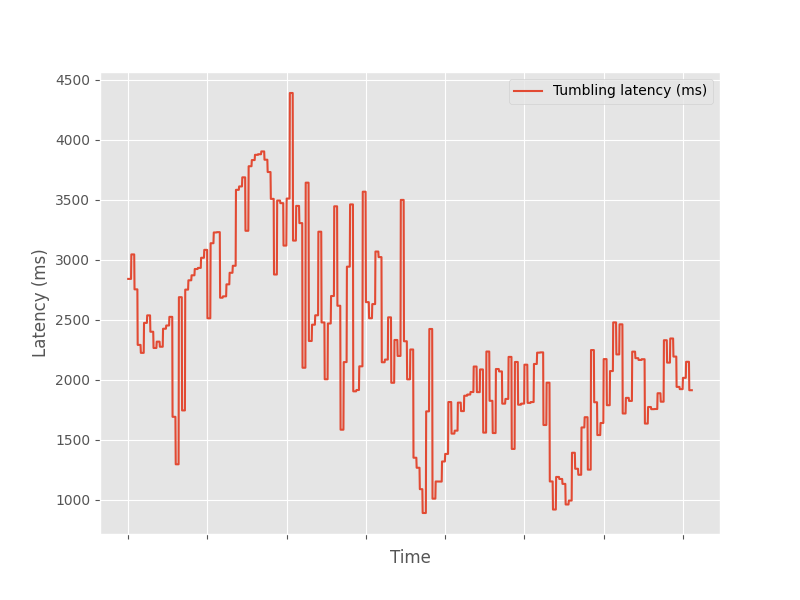
\includegraphics[width=\textwidth]{fig/periodic/Tumbling_latency_lineplot.png}
        \caption{Tumbling latency }
        \label{fig:periodic_tumbling_lineplot}
    \end{subfigure}
    \hfill
    \begin{subfigure}[b]{0.5\textwidth}
        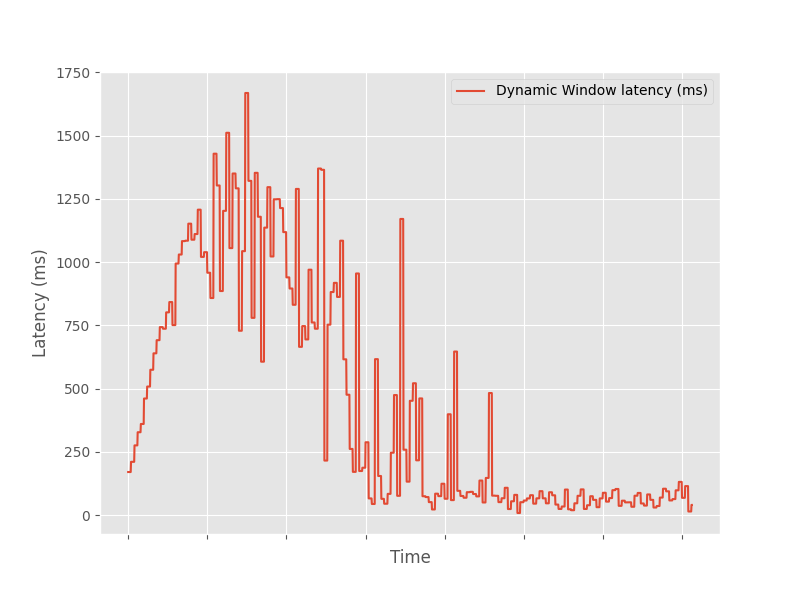
\includegraphics[width=\textwidth]{fig/periodic/DynamicWindow_latency_lineplot.png}
        \caption{Dynamic latency }
        \label{fig:periodic_dynamic_lineplot}
    \end{subfigure}
    \caption{Latency measurement of periodic workload over the lifetime of evaluation}
    \label{fig:periodic_latency_lineplot}
\end{figure*}

\begin{figure*}
    \begin{subfigure}[b]{0.5\textwidth}
        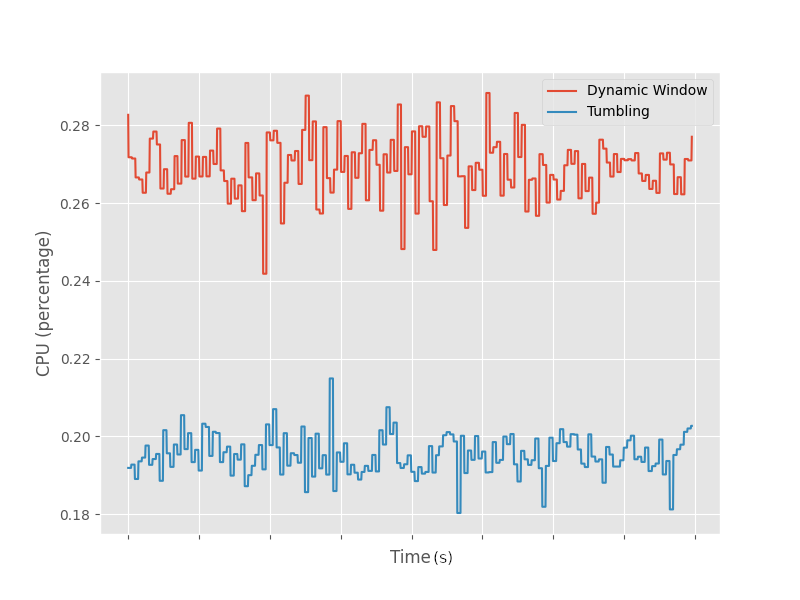
\includegraphics[width=\textwidth]{fig/periodic/cpu_comparison.png}
        \caption{CPU usage}
        \label{fig:periodic_cpu}
    \end{subfigure}
    \hfill 
    \begin{subfigure}[b]{0.5\textwidth}
        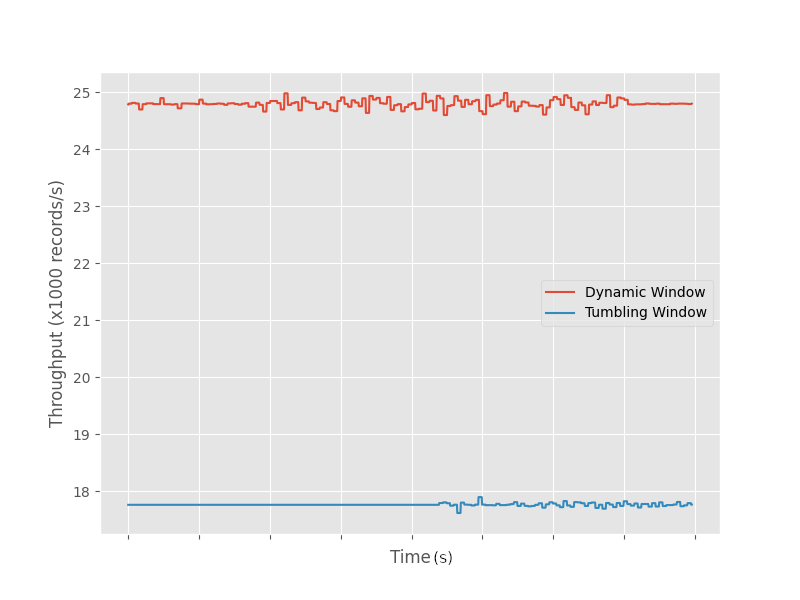
\includegraphics[width=\textwidth]{fig/periodic/throughput_comparison.png}
        \caption{Throughput of joined records}
        \label{fig:periodic_throughput}
    \end{subfigure}
    %%
    \begin{subfigure}[b]{0.5\textwidth}
        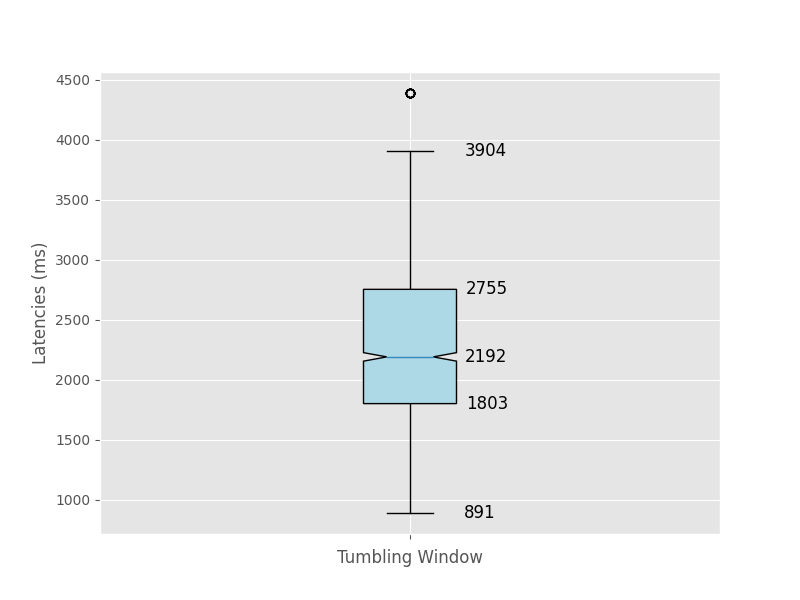
\includegraphics[width=\textwidth]{fig/periodic/TumblingWindow_latency_boxplot.png}
        \caption{Tumbling latency distribution}
        \label{fig:periodic_tumb_boxplot}
    \end{subfigure}
    \hfill 
    \begin{subfigure}[b]{0.5\textwidth}
        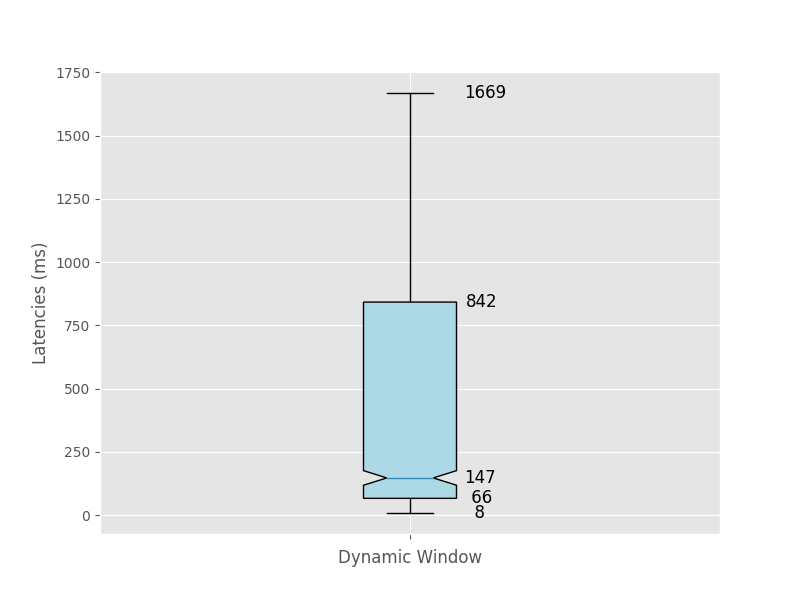
\includegraphics[width=\textwidth]{fig/periodic/DynamicWindow_latency_boxplot.png}
        \caption{Dynamic latency distribution}
        \label{fig:periodic_dynamic_boxplot}
    \end{subfigure}
    % 
    \begin{subfigure}[b]{\textwidth}
        \centering
        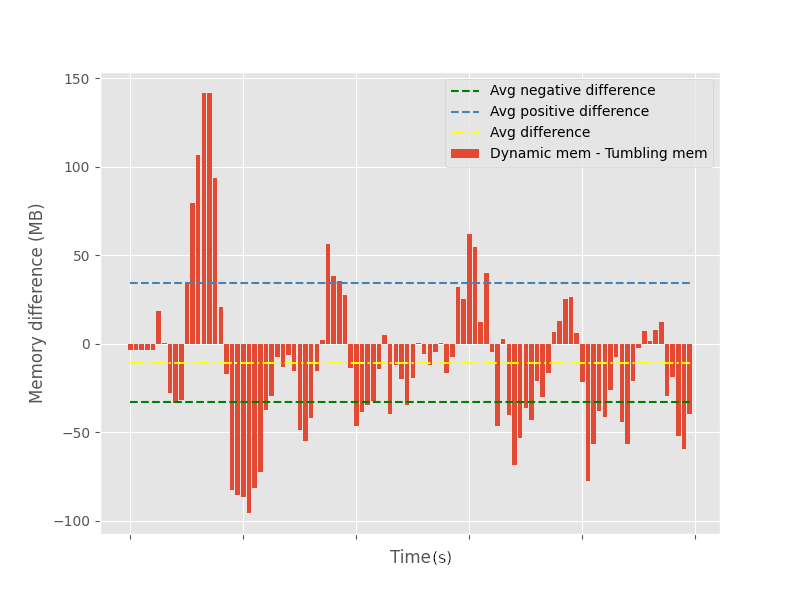
\includegraphics[width=0.5\textwidth]{fig/periodic/mem_difference_bar.png}
        \caption{Relative difference in memory usage from the perspective of dynamic window}
        \label{fig:periodic_mem_diff}
    \end{subfigure}

    \caption{Metrics measurements for periodic workload.}%
    \label{fig:periodic_measurement}
\end{figure*}

\newpage
\section{Workload for completeness measure}%
\label{sec:Workload for completeness measure}

From the results in Table~\ref{tab:dynamic_completeness}, and 
Table~\ref{tab:tumbling_completeness}, we could conclude that Dynamic window 
outperforms Tumbling window in terms of generating a more \emph{complete} output. 
Dynamic window has an IOU score of \textbf{1} for constant low stream rate
due to the subwindow sizes growing large 
enough to accommodate all the required records, to generate the \emph{complete} set 
of output. In contrast, Tumbling window scores only \textbf{0.749}, leading to 
a conclusion that a window size of 2s is not enough to process the low stream rate 
of the evaluation data. 

Similary for periodic burst input, Dynamic window outperforms Tumbling window with a
score of \textbf{0.982} whereas Tumbling window only scores \textbf{0.780}.   


\begin{table}[htbp]
    \centering
    \resizebox{\textwidth}{!}{%
\begin{tabular}{|r|r|r|r|r|}
\hline
\multicolumn{1}{|c|}{Stream rate} & \multicolumn{1}{c|}{Generated (triples)} & \multicolumn{1}{c|}{Expected (triples)} & \multicolumn{1}{c|}{Common (triples)} & \multicolumn{1}{c|}{\textbf{IOU score}} \\ \hline
Constant rate                     & 30,771,450                               & 30,771,450                              & 30,771,450                            & \textbf{1}                              \\ \hline
Periodic burst                    & 31,753,420                               & 32,319,110                              & 31,753,420                            & \textbf{0.982}                          \\ \hline
\end{tabular}%
}
\caption{Dynamic window's completeness measurement. The \emph{Expected (triples)} are the number of triples generated by the 
bounded data processing RMLStreamer.}
\label{tab:dynamic_completeness}
\end{table}

\begin{table}[htbp]
    \centering
    \resizebox{\textwidth}{!}{%
\begin{tabular}{|r|r|r|r|r|}
\hline
\multicolumn{1}{|c|}{Stream rate} & \multicolumn{1}{c|}{Generated (triples)} & \multicolumn{1}{c|}{Expected (triples)} & \multicolumn{1}{c|}{Common (triples)} & \multicolumn{1}{c|}{\textbf{IOU score}} \\ \hline
Constant rate                     & 23,059,350                               & 30,771,450                              & 23,059,350                            & \textbf{0.749}                              \\ \hline
Periodic burst                    & 24,412,150                               & 31,287,300                              & 24,412,150                            & \textbf{0.780}                          \\ \hline
\end{tabular}%
}
\caption{Tumbling window's completeness measurement. 
    The \emph{Expected (triples)} are the number of triples generated by the 
bounded data processing RMLStreamer.}
\label{tab:tumbling_completeness}
\end{table}



\chapter{Conclusion and Future Works}%
\label{chap:Conclusion and Future Works}


In this paper, we have presented an approach for Dynamic window 
which adapts its window size according to the stream rate of the 
input data sources. Our approach aims to fix the shortcomings of 
the existing state-of-the-art dynamic windowing approaches for 
join operator. We introduced a simple heuristic to adapt our 
window sizes dynamically without huge memory or computation overhead. 

We implemented our Dynamic window on top of the existing RMLStreamer, 
to evaluate its performance under a realistic processing environment. 
We adapted the benchmark framework as stated in~\cite{evalution_of_spe} to 
accurately evaluate the performance of our implementation against the 
standard fixed size Tumbling window under different stream characteristics. 

The results gathered from our evaluation concludes that our implementation 
of Dynamic window fares better than Tumbling window in terms of 
latency, throughput, and completeness with only a slight 
increase in CPU usage. Even though, we could not confidently conclude that 
the memory usage is lower in Dynamic window, our preliminary results indicate 
that it performs at worst case as bad as Tumbling window.   

Therefore, there are still areas of improvement to be made in terms of the
evaluation setups
and the dynamic algorithm. On the evaluation side, we could further increase 
the precision of our memory measurement by only counting the number of records
residing in the windows at any moment instead of the whole JVM heap of the RMLStreamer job. 
Furthermore, the evaluation could be done in the same benchmark pipelines as in~\cite{evalution_of_spe} 
to further evaluate the Dynamic window performance in a general stream processing use case instead 
of in the context of RDF mapping engines.  
Improvements on our dynamic approach could be achieved by allowing user to 
define other statistical approach 
to better calculate the threshold for adapting the window sizes. For example, one could provide 
RMLStreamer with an external function to calculate the metrics in Dynamic window similar to the approach 
in FnO~\cite{fno_ben}.
As an extension, a dynamic window based on \emph{count} could be of interest in use 
cases where \emph{timeliness} is not required but the number of elements is of importance.
Furthermore, utilizing mapping file to configure our window might also allow further
optimization in the mapping file for a more efficient mapping job as proposed in FunMap~\cite{funmap}. 




\printbibliography[heading=bibintoc]

% appendix
\appendix
\chapter{RML mapping specifications}

\section{Dynamic window join's RML mapping file}
\begin{lstlisting}[
    label={lst:dynamic_mapping_file}
    ]
@prefix rr: <http://www.w3.org/ns/r2rml#> .
@prefix foaf: <http://xmlns.com/foaf/0.1/> .
@prefix ex: <http://example.com/> .
@prefix xsd: <http://www.w3.org/2001/XMLSchema#> .
@prefix rml: <http://semweb.mmlab.be/ns/rml#> .
@prefix rmls: <http://semweb.mmlab.be/ns/rmls#> .
@prefix ql: <http://semweb.mmlab.be/ns/ql#> .
@prefix activity: <http://example.com/activity/> .
@prefix rdfs: <http://www.w3.org/2000/01/rdf-schema#>.
@prefix schema: <https://schema.org/>. 
@base <http://example.com/base/> .

_:kafka_source_ndwSpeed a rmls:KafkaStream ;
             rmls:broker "192.168.0.237:9092";
             rmls:groupId "1";
             rmls:topic "ndwspeed".

_:kafka_source_ndwFlow a rmls:KafkaStream ; 
            rmls:broker "192.168.0.237:9092"; 
            rmls:groupId "1"; 
            rmls:topic "ndwflow". 



<JoinConfigMap> a rmls:JoinConfigMap;
        rmls:joinType rmls:DynamicWindowJoin.


<NDWSpeedMap>
  a rr:TriplesMap;

  rml:logicalSource [
    rml:source _:kafka_source_ndwSpeed;
    rml:referenceFormulation ql:JSONPath; 
    rml:iterator "$"
  ];

  rr:subjectMap [
    rr:template "http://example.com/resource/{internalId}?lat={lat}&long={long}&speed={speed}&accuracy={accuracy}&timestamp={timestamp}"
  ];

  
  rr:predicateObjectMap [
    rr:predicate <http://example.com/ontology/laneFlow> ;
    rr:objectMap [
      rr:parentTriplesMap <NDWFlowMap>;
      rmls:joinConfig <JoinConfigMap>;
      rmls:windowType  rmls:DynamicWindow;
      rr:joinCondition [
        rr:child "internalId,lat,long,timestamp" ;
        rr:parent "internalId,lat,long,timestamp" ;
      ]
    ]
  ] .

<NDWFlowMap>
  a rr:TriplesMap;
  rml:logicalSource [
    rml:source _:kafka_source_ndwFlow;
    rml:referenceFormulation ql:JSONPath;
    rml:iterator "$"
  ];



  rr:subjectMap [
    rr:template "http://example.com/resource/{internalId}?lat={lat}&long={long}&flow={flow}&period={period}&accuracy={accuracy}&timestamp={timestamp}"
  ]. 
\end{lstlisting}

\section{Tumbling window join's RML mapping file}
\begin{lstlisting}[label={lst:tumbling_mapping_file}]
@prefix rr: <http://www.w3.org/ns/r2rml#> .
@prefix foaf: <http://xmlns.com/foaf/0.1/> .
@prefix ex: <http://example.com/> .
@prefix xsd: <http://www.w3.org/2001/XMLSchema#> .
@prefix rml: <http://semweb.mmlab.be/ns/rml#> .
@prefix rmls: <http://semweb.mmlab.be/ns/rmls#> .
@prefix ql: <http://semweb.mmlab.be/ns/ql#> .
@prefix activity: <http://example.com/activity/> .
@prefix rdfs: <http://www.w3.org/2000/01/rdf-schema#>.
@prefix schema: <https://schema.org/>. 
@base <http://example.com/base/> .

_:kafka_source_ndwSpeed a rmls:KafkaStream ;
             rmls:broker "192.168.0.237:9092";
             rmls:groupId "1";
             rmls:topic "ndwspeed".

_:kafka_source_ndwFlow a rmls:KafkaStream ; 
            rmls:broker "192.168.0.237:9092"; 
            rmls:groupId "1"; 
            rmls:topic "ndwflow". 



<JoinConfigMap> a rmls:JoinConfigMap;
        rmls:joinType rmls:TumblingWindowJoin.


<NDWSpeedMap>
  a rr:TriplesMap;

  rml:logicalSource [
    rml:source _:kafka_source_ndwSpeed;
    rml:referenceFormulation ql:JSONPath;
    rml:iterator "$"
  ];

  rr:subjectMap [
    rr:template "http://example.com/resource/{internalId}?lat={lat}&long={long}&speed={speed}&accuracy={accuracy}&timestamp={timestamp}" 
  ];

  rr:predicateObjectMap [
    rr:predicate <http://example.com/ontology/laneFlow> ;
    rr:objectMap [
      rr:parentTriplesMap <NDWFlowMap>;
      rmls:joinConfig <JoinConfigMap>;
      rmls:windowType  rmls:Tumbling;
      rr:joinCondition [
        rr:child "internalId,lat,long,timestamp" ;
        rr:parent "internalId,lat,long,timestamp" ;
      ]
    ]
  ] .

<NDWFlowMap>
  a rr:TriplesMap;
  rml:logicalSource [
    rml:source _:kafka_source_ndwFlow;
    rml:referenceFormulation ql:JSONPath;
    rml:iterator "$"
  ];

  rr:subjectMap [
    rr:template "http://example.com/resource/{internalId}?lat={lat}&long={long}&flow={flow}&period={period}&accuracy={accuracy}&timestamp={timestamp}"
  ].
\end{lstlisting}

\section{Bounded data join RML mapping file}
\begin{lstlisting}[label={lst:bounded_mapping_file}]
@prefix rr: <http://www.w3.org/ns/r2rml#> .
@prefix foaf: <http://xmlns.com/foaf/0.1/> .
@prefix ex: <http://example.com/> .
@prefix xsd: <http://www.w3.org/2001/XMLSchema#> .
@prefix rml: <http://semweb.mmlab.be/ns/rml#> .
@prefix rmls: <http://semweb.mmlab.be/ns/rmls#> .
@prefix ql: <http://semweb.mmlab.be/ns/ql#> .
@prefix activity: <http://example.com/activity/> .
@prefix rdfs: <http://www.w3.org/2000/01/rdf-schema#>.
@prefix schema: <https://schema.org/>. 
@base <http://example.com/base/> .


<NDWSpeedMap>
  a rr:TriplesMap;

  rml:logicalSource [
    rml:source "ndwspeed.json" ;
    rml:referenceFormulation ql:JSONPath; 
    rml:iterator "$.*"
  ];

  rr:subjectMap [
    rr:template "http://example.com/resource/{internalId}?lat={lat}&long={long}&speed={speed}&accuracy={accuracy}&timestamp={timestamp}"
  ];

  
  rr:predicateObjectMap [
    rr:predicate <http://example.com/ontology/laneFlow> ;
    rr:objectMap [
      rr:parentTriplesMap <NDWFlowMap>;
      rr:joinCondition [
        rr:child "internalId,lat,long,timestamp" ;
        rr:parent "internalId,lat,long,timestamp" ;
      ]
    ]
  ] .

<NDWFlowMap>
  a rr:TriplesMap;
  rml:logicalSource [
    rml:source "ndwflow.json";
    rml:referenceFormulation ql:JSONPath;
    rml:iterator "$.*"
  ];



  rr:subjectMap [
    rr:template "http://example.com/resource/{internalId}?lat={lat}&long={long}&flow={flow}&period={period}&accuracy={accuracy}&timestamp={timestamp}"
  ]. 
\end{lstlisting}


% add appendix


\backmatter

% optional: list figures/tables
%\listoffigures
%\listoftables

\end{document}
